\documentclass[letterpaper, 12pt, parskip=full,DIV=10]{scrartcl}
% The next three lines are temporary, for todo notes, remove after notes are removed
%\documentclass[letterpaper, 12pt, parskip=full,]{scrartcl}
%\setlength{\marginparwidth}{4.5cm}
%\usepackage[top=2.5cm, bottom=2.5cm, left=1.5cm, right=5cm]{geometry}
\input{../preanalysis/template_MOW.sty}

\title{Battling the Coronavirus ``Infodemic'' Among Social Media Users in Africa}
%\subtitle{}
\author[1]{Molly Offer-Westort}
\author[2]{Leah R. Rosenzweig}
\author[3]{Susan Athey}
\affil[1]{Department of Political Science, University of Chicago; mollyow@uchicago.edu}
\affil[2]{Development Innovation Lab, University of Chicago}
\affil[3]{Stanford Graduate School of Business, Stanford University}
\date{\today}


\usepackage{titletoc}
\usepackage{siunitx}

\begin{document}%
\normalsize%
\maketitle%

%%%%%%%%%%%%%%%%%%%%%%%%%%%%%%%%%%%%%%%%%%%%
%FRONTMATTER
%%%%%%%%%%%%%%%%%%%%%%%%%%%%%%%%%%%%%%%%%%%%

\textbf{Author Contributions: }

\textbf{Competing Interest Statement: }\todo{add note with link to anonymized preanalysis plan}

\textbf{Classification:} \todo{Paste the major and minor classification here. Dual classifications are permitted, but cannot be within the same major classification.}

\textbf{Keywords (3-5):} Misinformation - covid - adaptive experiment

%% for nature human behavior:
%Main text – up to 5,000 words, excluding abstract, Methods, references and figure legends.
%Abstract – up to 150 words, unreferenced. 
%Display items – up to 8 items (figures and/or tables). 
%Article should be divided as follows: 
%Introduction (without heading) 
%Results (concise, focused account of the findings)
%Discussion
%Methods. ​



{\textbf{Abstract:}}
\begin{abstract} %150 words for nature human behavior (currently over by ~10)
Using an adaptive experiment with Facebook users recruited on the platform in Kenya and Nigeria, we tested 40 combinations of interventions with the goal of improving sharing discernment regarding COVID-19-related posts. We found common approaches used by social media platforms, such as flagging misleading posts or including related articles, to be ineffective, and estimate precise null effects of these treatments. Instead, providing tips for spotting misinformation and nudging users to think about the accuracy of media content improves sharing discernment -- reducing intended sharing of false posts without adversely affecting true posts. Providing tips leads to effects equivalent to a nearly 8\% reduction in intended sharing of false information, and nudging accuracy to a 4\% reduction.  Both interventions are successful among some of the worst offenders, who intend to share more false news at baseline. % -- specifically men, users with lower digital literacy, and less scientific knowledge.
\textcolor{green}{We also find significant differences in response to these treatments across users, indicating differences in mechanisms through which the interventions affect outcomes. }\todo{MOW: tried something here}
The results suggest that these low-cost scalable interventions can significantly improve the quality of information circulating online.

 
\end{abstract}

\textbf{Significance statement:}
Health misinformation can be deadly. Alongside the global coronavirus pandemic there has been an ``infodemic'' of rumors about the virus and hoax cures.  Which online interventions delivered via social media help to limit the spread of misinformation? We experimentally evaluated a slate of interventions to learn which are effective at reducing social media users' intentions to share false information about COVID-19. Warning labels on posts had little influence while accuracy prompts and tips had positive effects in both countries. The results suggest that platforms may wish to consider implementing these low-cost scalable interventions to reduce sharing of misinformation globally. 


\clearpage

%%%%%%%%%%%%%%%%%%%%%%%%%%%%%%%%%%%%%%%%%%%%
%INTRODUCTION
%%%%%%%%%%%%%%%%%%%%%%%%%%%%%%%%%%%%%%%%%%%%

\section{Introduction}

% context / problem area
Alongside the outbreak of the novel coronavirus (SARS-CoV-2), much of the world's population also experienced an ``infodemic''---the spread of misinformation related to the virus. Like the actual virus, COVID-19 misinformation is not bounded by state borders. Although other forms of false information have been shown to spread faster and farther than corresponding true information \citep{vosoughi2018spread}, early evidence indicates that COVID-19 information from reliable and questionable sources did not differ in their spread \citep{cinelli2020covid}.  Other work on COVID-19 conspiracy theories, specifically, suggests that these rumors were more viral than neutral or debunking stories \citep{HKS_whatsapp}.  %COVID-19 may follow the trajectory of other types of online information, where false information spreads faster and farther than true information \citep{vosoughi2018spread}. For instance, misinformation about the Zika virus was three times more likely to be shared on social media than verified information on several social media sites \citep{sharma2017zika}.  Of course, the difference lies in the potential effects of the spread of the information -- the spread of COVID-19 misinformation puts more lives at risk.  
Regardless of its speed and reach, COVID-19 misinformation presents a challenge for policy makers trying to keep their citizens safe.  % lots of types of misinfo dangerous - most dangerous = hoax cures...

% specific problem / question + real world importance
Before effective vaccines were developed and widely available people across the globe looked to alternative sources for prevention techniques and remedies for COVID-19, which have proven to be deadly. In Nigeria, multiple people were hospitalized for chloroquine poisoning following statements by former president Trump suggesting the medication could be used to treat COVID-19 \citep{busari2020nigeria}. In Iran, dozens of people died from alcohol poisoning after ingesting methanol supposedly due to the rumor that alcohol could prevent coronavirus \citep{haghdoost2020alcohol}. Particularly in contexts with weak healthcare systems, the uncertainty over how to combat COVID-19 infection may have been particularly daunting and the search for remedies that much more urgent. %have been likely candidates for viral shares in the early stages of the pandemic when mortality rates were high and a vaccine did not yet exist.


% our study - what we do / contribute
This paper focuses on these particularly dangerous pieces of COVID-19 misinformation -- hoax ``cures'' -- and tests numerous online interventions designed to curb the spread of these falsities, while not adversely affecting the sharing of true information on COVID-19 prevention techniques.  We began this study in February 2021 before vaccines were widely available. Using targeted Facebook advertisements, we recruited a sample of social media users living in Kenya and Nigeria, two of the three largest Facebook markets in sub-Saharan Africa \citep{world-population-reviewfacebook}. Using a Facebook Messenger chatbot,  we engaged participants in a survey experiment that recruited and kept these social media users on the platform where they might naturally engage with similar media posts, to enhance the realism of the study.  Participants answered survey questions and were randomized into different treatments delivered by the Messenger chatbot. Our main outcome of interest is sharing discernment -- whether respondents indicate wanting to share true but not false posts. 


% sharing = outcome of interest
This paper focuses on sharing, rather than belief, since exposure can further false narratives through resharing even if it doesn't affect an individual's belief. And misinformation can have harmful effects, regardless of the motivation for sharing: there is suggestive evidence that the spread of misinformation is correlated with behavior. One study analyzed more than 100 million Twitter posts worldwide and found a correlation between waves of unreliable information prior to a rise in COVID-19 infections \citep{gallotti2020assessing}. Another study of Fox News viewers in the US demonstrates that greater exposure to COVID-19 misinformation is associated with lower adoption of preventative behaviors \citep{bursztyn2022opinions}. Randomized controlled trials also find that exposure to COVID-19 misinformation lowers intentions to engage in physical distancing among a convenience sample of German university students \citep{pummerer2022conspiracy} and intentions get the vaccine among nationally representative samples in the US and UK \citep{loomba2021measuring}.


%intention - behavior gap - concerns of experimenter demand bias. survey exp. not field exp. 

% our contributions / benefit over other similar studies - in context of general limitations re. external validity

This study, like others focused on online misinformation, faces several limitations related to external validity. First, our goal is to identify interventions that are effective among average social media users. We are limited, however, in our recruitment methods to engaging with those who clicked on our Facebook ads to participate in the study.  Recruiting actual social media users on the platform improves beyond convenience samples, laboratory experiments, and opt-in survey panels.  But we cannot say how users who decided to participate in our study might differ on unobservables to the general population of Facebook users in these countries. Importantly, this study brings comparative data to this global question which is most often studied using samples recruited from Qualtrics, Lucid, or MTurk in North America.  

% survey experiment 
Second, interacting with participants of a study and delivering interventions in the course of a survey experiment is an imperfect proxy for understanding how users would react to real interventions delivered on the platform.  Though still artificial, our approach of delivering the survey and interventions through a Facebook Messenger chatbot provides greater realism than interventions delivered on other platforms like Qualtrics.  The nature of our survey experiment means that participants were aware they were part of a study (rather than an on-platform field experiment, for example,  where consent may be waived by IRB or implicitly provided when users agree to the terms and conditions). Thus, it is possible that participants may be responding in particular ways due to experimenter demand effects. The validity of our results would be called into question if participants gleaned the intention of the study and adjusted their responses to match what they thought the researchers wanted to hear, rather than reflecting how they truly believed or wanted to behave.  \textcolor{red}{Later we presents tests that suggest our results are not wholly driven by experimenter demand bias.} \todo{MOW: not in here yet, currently referenced on p. 14. }

%sharing outcome 
Finally, misinformation studies that focus on sharing behavior as the main outcome of interest are inherently limited by ethical concerns of not wanting to contribute to the ecosystem of misinformation by allowing survey participants to \textit{actually share} false posts. We,  like many others, instead use measures of sharing \textit{intentions}.  While scholars have found that intentions are correlated with actual online sharing behavior \citep{mosleh2020self}, measuring intentions rather than actual sharing behavior remains a main limitation of scholarship in this area.  In this study, we directly ask participants ``Do you want to share this post on your timeline/on Messenger?,'' rather than phrasing it as a hypothetical question. We simultaneously told participants not to share the post now, but they would be able to do so at the end of the study. When we debriefed respondents at the end of the study, we told them which posts they saw were false and explained that was why they could not share those posts. We gave participants an opportunity to share the true posts they had said they wanted to share. \todo{We should check this is correlated with true sharing intentions.} A unique contribution of this study is that for each post (true and false), we asked participants if they wanted to share it on Timeline (public to their friends on Facebook) or on Messenger (a direct private message). We observe variation in sharing preferences by channel that suggest participants are discerning in their stated sharing intentions for true and false posts at baseline. 


%This study aimed to understand what online interventions might be effective at curbing the spread of hoax COVID ``cures'' on social media among users in two African countries. Several challenges exist in trying to answer this question without access to on-platform experimentation. 


% interventions
To curb sharing of false posts we examine interventions delivered to both the individual user, such as tips for spotting fake news and nudges; as well as treatments delivered alongside specific posts, such as flags or warning labels pinned alongside the article of interest. Evaluating both types of interventions -- those targeting users and those associated with individual posts -- alongside one another is important give how much these different strategies vary in their cost and scalability. Interventions that flag specific posts rely on time and resource intensive fact-checking sources to verify the veracity of individual posts before applying such labels.  General interventions delivered to users while they are on a particular platform, on the other hand, are less resource intensive and much more easily delivered en masse. 

Traditional randomized experiments are often limited by the number of interventions due to power considerations, but our adaptive design allows us to sort through numerous interventions.  Drawing on behavioral science theory and industry practice, we \textcolor{green}{used a multi-factorial adaptive design to} evaluate the effectiveness of seven respondent-level interventions and four headline-level interventions during an adaptive learning phase. These interventions speak to the debate as to whether misinformation spreads because people are not paying enough attention or people do not have skills to spot it.  We find evidence in support of both theories, and our results suggest that interventions targeting individuals rather than specific posts are more effective overall. 


% specific research questions / contributions - play up design and the more nuanced targeting questions we ask/answer
% maybe use this par as outline par - if results section comes next - outline subsections of results...
This paper investigates several important questions.  Do social media users have different preferences for how they share true and false posts about COVID-19? Can we identify interventions that are effective at reducing the sharing of false information, without adversely affecting sharing of true information? We also explore whether there are benefits to policy targeting from two perspectives. First, we analyze which recipients should be targeted with interventions. Second, we observe whether particular interventions should be designated for certain types of users and not for others.  \textcolor{red}{This study is able to take a more comprehensive approach toward subgroup analysis by exploring who shares the most misinformation at baseline and who is most affected by treatment looking at covariates academic studies have found to be significant predictors, as well as characteristics platforms collect on users. }With the goal of minimizing the spread of misinformation in the online information ecosystem, we quantify the best approach in this setting and offer lessons for other contexts.


%%%%%%%%%%%%%%%%%%%%%%%%%%%%%%%%%%%%%%%%%%%%
%MATERIALS AND METHODS
%%%%%%%%%%%%%%%%%%%%%%%%%%%%%%%%%%%%%%%%%%%%

\section{Materials and Methods}
\subsection{Design}
Our study was conducted in two stages; a ``learning'' stage, which ran from Febrary 26 - March 22, 2021, in which we used a multi-factorial contextual adaptive experimental design to learn optimal interventions, and an ``evaluation'' stage (June 30 - July 20, 2021)\todo{confirm dates}, in which we compared only the most effective interventions established in the learning stage to obtain precise estimation of their effects. 

We considered two types of interventions: seven respondent-level interventions and four headline-level interventions. The respondent-level interventions included behavioral nudges and trainings targeted to the the participants themselves: tips and trainings to spot false news (from Facebook, AfricaCheck, and a BBC video), an emotion suppression prompt, an accuracy nudge, and a pledge that participants took to keep their family and friends safe. The headline-level interventions were applied to the headlines or posts themselves: a flag for articles that had been fact checked by third-party websites, links to further information, or accompanied by additional related articles or countering information from a validated source such as the WHO. Table~\ref{tab:treatments} in the Supplementary Information (SI) describes all of the interventions we tested. Section~\ref{appendix:learning} in the SI discusses learning stage design and results.  The two respondent-level  and two headline-level treatments that were found to be most effective in the learning phase include an accuracy nudge and Facebook trips (respondent-level) and factcheck and related articles (headline-level), which are presented in Figure~\ref{fig:treatments}.


\begin{figure}[H]
\centering
\begin{tabular}{%
@{\hspace{0\tabcolsep}}p{0.25\textwidth}%
@{\hspace{0\tabcolsep}}p{0.25\textwidth}%
@{\hspace{0\tabcolsep}}p{0.25\textwidth}%
@{\hspace{0\tabcolsep}}p{0.25\textwidth}}
\includegraphics[width=0.25\textwidth]{../analysis/figures/accuracy_short.png}  & 
\includegraphics[width=0.25\textwidth]{../analysis/figures/fb_tips.png} & 
\includegraphics[width=0.25\textwidth]{../analysis/figures/factcheck.png}  & 
\includegraphics[width=0.25\textwidth]{../analysis/figures/our_related_articles.png} \\
\hfil\textbf{Accuracy} &  \hfil\textbf{Facebook Tips} &\hfil \textbf{Factcheck} & \hfil \textbf{Related Articles}
%\\
% \multicolumn{2}{c}{\textbf{Respondent:} delivered before posts} & 
% \multicolumn{2}{c}{\textbf{Headline:} delivered as part of post}
\end{tabular}
\caption{\textbf{Respondent- and headline-level treatments tested in the evaluation phase.}}
\label{fig:treatments}
\end{figure}

\subsection{Outcome measures}\label{section:measures}
Our outcome measures capture discernment in sharing intentions. We show participants a series of real social media posts about COVID-19 cures, treatments, and preventative best practices and ask if they wanted to share the post.  The stimuli include both true information, sourced from the WHO, the Nigeria Center for Disease Control, the National Emergency Response Committee in Kenya, and the Ministry of Health in both countries. The false posts were sourced from AFP, Poynter, and AfricaCheck websites lists of misinformation that had appeared online and was fact-checked in Kenya and Nigeria since the start of the pandemic.  Each participants saw four post-treatment stimuli, two true and two false in a random order. For each stimuli, we asked respondents two questions: if they wanted to share it (privately) in Facebook Messenger and if they wanted to share it (publicly) on their Timeline. 

\subsubsection{Combined response measure}
In the learning portion of the experiment, our adaptive algorithm updated based on a combined outcome measure, pre-registered in our design document. This measure is the summed number of times users said they would like to share true and misinformation stimuli respectively over Facebook Messenger and on their Facebook Timeline, across two stimuli of each type. Users could share each type of stimuli up to four times (two channels of sharing x two stimuli). As our aim is to learn treatments that will decrease sharing of false information while not overly harming sharing of true information, false posts are given a weight of -1, and true posts are given a weight of 0.5 in this measure. \todo{LR: helpful to put table of potential values of response funct here? might make later tables/figs easier to interpret?}

\begin{table}[!ht]
\centering
\begin{tabular}{lrrrrrr}
                                   & & \multicolumn{5}{c}{\textbf{True shares}}     \\ 
                                   & & 0                    & 1                    & 2                                 & 3                    & \multicolumn{1}{r}{4}    \\  \cmidrule(lr){3-7}
\multicolumn{1}{l}{}              & \multicolumn{1}{r}{0} & 0.0                  & 0.5                  & 1.0                               & 1.5                  & \multicolumn{1}{r}{2.0}  \\
\multicolumn{1}{l}{}              & \multicolumn{1}{r}{1} & -1.0                 & -0.5                 & 0.0                               & 0.5                  & \multicolumn{1}{r}{1.0}  \\
\multicolumn{1}{l}{\textbf{False shares}} & \multicolumn{1}{r}{2} & -2.0                 & -1.5                 & -1.0                              & -0.5                 & \multicolumn{1}{r}{0.0}  \\
\multicolumn{1}{l}{}              & \multicolumn{1}{r}{3} & -3.0                 & -2.5                 & -2.0                              & -1.5                 & \multicolumn{1}{r}{-1.0} \\
\multicolumn{1}{l}{}              & \multicolumn{1}{r}{4} & -4.0                 & -3.5                 & -3.0                              & -2.5                 & \multicolumn{1}{r}{-2.0} \\ 
\end{tabular}
\caption{\textbf{Combined response measure.}}
\label{tab:response_fun}
\end{table}

\subsubsection{Sharing disaggregated by true and false stimuli, and by sharing channel}
For our primary reporting, we report results for both types of stimuli separately, for improved interpretability and to better illustrate how the treatments affect sharing discernment. For this measure, we calculate the proportion of true and false stimuli respondents reported intending to share, across either Messenger or timeline. We also report sharing disaggregated by channel (Messenger, timeline).  

\subsection{Survey recruitment}
We conducted this study with social media users in Kenya and Nigeria, two major English-language hubs of online communication in East and West Africa, respectively. Kenya and Nigeria also represent two of Facebook's top three largest user bashes in sub-Saharan Africa \citep{africa2016top}, with a combined user base of 30-35 million users ages 18 years and older.%
\footnote{
Reported on the audience insights tool on Facebook's advertising platform.%
} We recruited social media users 18 years and over in these countries through targeted Facebook advertisements (see Figure~\ref{fig:recruitment} in the SI) \citep{Rosenzweig_2020}.  Users who clicked on our ads then started a conversation with our page's Messenger chatbot. \footnote{The ads and experiment were carried out using the Facebook page Social Impact Research Initiative (\url{https://www.facebook.com/socialimpactresearchlab}).}

\subsection{Estimating procedures}\label{section:estimation}
For individuals indexed by $i$, we observe covariates $X_i$, and use an assignment procedure to assign categorical treatments $W_i \in \W$. Observed response for individual $i$ is represented by $Y_i$. We denote the outcome for individual $i$ under treatment $w$ as $Y_i(w)$. Treatment assignment probabilities are represented by $e_i(w):=\Pr[W_i=w\rvert X_i=x]$. To estimate average response under counterfactual treatment conditions and average treatment effects, we use a generalized augmented inverse probability weighted estimator \citep{robins1994estimation}. To account for non-normality of the estimator on adaptively collected data, we use adaptive weights, described in \cite{zhan2021off}.%
\footnote{
The scores for the augmented inverse probability weighted estimator are calculated as
\begin{equation}
\Gamma^{AIPW}_i(w) := \hat \mu_i (X_i; w) + \frac{\textbf{1}\{W_i = w\}}{e_i(X_i;w)}\left(Y_i - \hat\mu_i(X_i;w) \right),
\end{equation}
where $\hat \mu_i (X_i; w)$ is a conditional means model, which we estimate using a random forest as implemented by the \texttt{grf} page in R statistical software \citep{Tibshirani:2020aa}. 
For the learning data, the AIPW scores are weighted using evaluation weights, $h_i(w)$,
\begin{equation}
Q_i^{h}(w) := \frac{ \frac{1}{N}\sum_{i = 1}^N h_i(w)\Gamma_i(w)}{\sum_{i = 1}^N h_i(w)} . 
\label{eq:scores_learning}
\end{equation}
We use the contextual stabilized variance weights described by \cite{zhan2021off}. 
For the evaluation data, we aggregate scores to estimate $\textrm{E}[Y_i(w)]$ as,
\begin{equation}
Q_i^{AIPW}(w) := \frac{1}{N}\sum_{i = 1}^N \Gamma^{AIPW}_i(w). 
\end{equation}
Contrasts are estimated by taking differences in (weighted) scores; estimation of standard errors follows the implementation in \cite{Tibshirani:2020aa}.%
}
Covariates used for adjustment are described in further detail in Table~\ref{tab:cov_long}. 



%%%%%%%%%%%%%%%%%%%%%%%%%%%%%%%%%%%%%%%%%%%%
%RESULTS
%%%%%%%%%%%%%%%%%%%%%%%%%%%%%%%%%%%%%%%%%%%%

\section{Results}
\subsection{Main effects}
Using data from the learning stage (see \hyperref[SI]{Supplementary Information}), we selected four treatments to test independently in the evaluation stage in addition to the pure control---two respondent-level, \textit{accuracy} and \textit{Facebook tips} and two headline-level, \textit{factcheck} and \textit{related articles} (see Figure~\href{x}). These were the treatments associated with the highest mean responses in each class separate from control, as estimated with the estimator described in Equation~\ref{eq:scores_learning}. We also learned an optimal contextual policy, assigning the most effective of the two respondent-level treatments based on individual covariate profiles. This policy is described in further detail in Section~\ref{section:het_policy}.  

Prior to collecting the evaluation data, we learned a contextual policy based on the combined response function, described in Section~\ref{section:measures}. This optimal contextual policy did not measurably improve the combined response over the two fixed respondent-level policies, and directionally was inferior in decreasing false sharing intentions as compared to Facebook tips. We report outcomes for this policy in Section~\ref{appendix:learning} in the supplementary information. To explore the additional benefits of accounting for context with the goal of decreasing false sharing intentions, we report in the main paper results with respect to a policy learned on the false sharing measure only. 

\subsubsection{Respondent-level treatments}
Considering the respondent-level treatments, the accuracy treatment asked participants to tell us whether they thought a separate post, unrelated to COVID, was accurate or not \citep{pennycook2020fighting}. The Facebook tips treatment provided participants with ten tips Facebook provides for how to be smart about what information to trust. These tips include being skeptical of headlines, watching for unusual formatting, checking the evidence, and looking at other reports, among others. The full text of the Facebook Tips treatment is presented in the Supporting Information. 

These treatments relate to two schools of thought as to why people are susceptible to misinformation.%
\footnote{
 There are of course additional theories to explain why people are susceptible to or share misinformation---for instance for identity-based or ideological reasons \citep{nyhan2010corrections}. These theories are not the focus of this study, however, and although we did ask about partisanship we do not see substantive differences in treatment effects by party ID.% 
}
The first from cognitive science suggests that people consume social media content quickly, react intuitively and do not stop to think about whether something is true or false. This reasoning suggests that people need to be reminded or ``nudged'' to consider the accuracy of posts, otherwise it may not be something they consider before sharing a post \citep{pennycook2021shifting}. A second reasoning suggests that people simply do not know how to identify misinformation. This theory prescribes providing training or tips to equip individuals to be able to spot misinformation in their news feed. Importantly, these are not mutually exclusive theories and people may suffer from both challenges---but whether one intervention is more successful, on average, than the other is important to understand as well as for which types of people one prescription may be better than the other. 

\subsubsection{Headline-level treatments}
We also evaluated two headline-level treatments. We used a factcheck intervention that has been used by several platforms and adds ``disputed'' flags to false posts, and we tested the related articles intervention that Facebook has used in the past---providing links to related articles under misleading or false posts \citep{ghosh2017facebook}.

Warning labels on posts have been found to be effective at helping users identify misinformation \citep{clayton2020real} and reduce individual's willingness to share fake-news headlines \citep{mena2020cleaning} in the context of political information. For COVID-19 information, \citet{kreps2020medical} find the effectiveness of these tags to depend on context, and worked for only one out of three false COVID headlines they tested. Recent evidence suggests fact checks can improve discernment (belief) in diverse contexts \citep{porter2021global}. \citet{brashier2021timing} also find that timing matters---specifically that debunking misinformation after the headline is shown was more successful than contemporaneous tags, but do not test how these flags and warnings affect sharing behavior. 

\subsubsection{Findings}

Table~\ref{tab:main_results} shows results for the evaluation phase under the pre-registered combined response function, as well as disaggregated by any intention to share false and true stimuli by either channel, and false and true sharing intentions by each channel. Our objective is to decrease intentions to share false information, while minimizing negative effects on intentions to share true information. To this end, we hope to see positive treatment effects for our combined response function, negative treatment effects on false sharing, and positive or neutral treatment effects on true sharing. 

\begin{table}[H]
\centering
\resizebox{\textwidth}{!}{ 
\begin{tabular}{lccccccc}
&    & \multicolumn{3}{c}{\textbf{False}} & \multicolumn{3}{c}{\textbf{True}} \\
& \textbf{Combined}& Any sharing & Messenger & Timeline & Any sharing & Messenger & Timeline \\
 \cmidrule(lr){2-2}  \cmidrule(lr){3-5}  \cmidrule(lr){6-8}
\multicolumn{4}{l}{\textbf{Headline treatment effects}} \rule{0pt}{1.2\normalbaselineskip}\\                            
\hspace{1em} Factcheck   & \num{-0.032} & \num{-0.005} & \num{-0.004} & \num{-0.005} & \num{-0.003} & \num{-0.001} & \num{-0.012}\\
 & (\num{0.036}) & (\num{0.012}) & (\num{0.011}) & (\num{0.011}) & (\num{0.011}) & (\num{0.012}) & (\num{0.012})\\
 \hspace{1em} Related articles   & \num{-0.054} & \num{0.008} & \num{0.002} & \num{0.009} & \num{-0.019} & \num{-0.012} & \num{-0.021}\\
 & (\num{0.035}) & (\num{0.012}) & (\num{0.011}) & (\num{0.011}) & (\num{0.011}) & (\num{0.012}) & (\num{0.012})\\
\multicolumn{4}{l}{\textbf{Respondent treatment effects}}\rule{0pt}{1.2\normalbaselineskip} \\                            
\hspace{1em} Accuracy  & \num{0.060}* & \num{-0.020}* & \num{-0.018}* & \num{-0.026}** & \num{-0.001} & \num{0.005} & \num{-0.011}\\
 & (\num{0.032}) & (\num{0.010}) & (\num{0.010}) & (\num{0.009}) & (\num{0.010}) & (\num{0.010}) & (\num{0.010})\\
\hspace{1em} Facebook tips   & \num{0.046}+ & \num{-0.033}** & \num{-0.029}** & \num{-0.030}** & \num{-0.016} & \num{-0.005} & \num{-0.022}\\
 & (\num{0.035}) & (\num{0.011}) & (\num{0.011}) & (\num{0.010}) & (\num{0.011}) & (\num{0.012}) & (\num{0.011})\\
\hspace{1em} Optimal   &  \num{0.073}* & \num{-0.039}*** & \num{-0.038}*** & \num{-0.032}*** & \num{-0.019} & \num{-0.012} & \num{-0.022}\\
 & (\num{0.034}) & (\num{0.011}) & (\num{0.010}) & (\num{0.010}) & (\num{0.011}) & (\num{0.011}) & (\num{0.011})\\
  \hline
  Control mean  & \num{-0.391} & \num{0.442} & \num{0.395} & \num{0.369} & \num{0.651} & \num{0.561} & \num{0.593}\\
 & (\num{0.027}) & (\num{0.009}) & (\num{0.008}) & (\num{0.008}) & (\num{0.008}) & (\num{0.009}) & (\num{0.009}) \\
\end{tabular}
\vspace{1ex}

}
\caption{\textbf{Control response and treatment effect estimates.} The last row represents estimated mean response under the control condition; all other rows are estimated treatment effects in contrast with the control condition. Estimates are produced from an augmented inverse probability weighted estimator, as described in Section~\ref{section:estimation}. $n = 10,681$. For contrasts only, \textsuperscript{+} $p<0.1$, \textsuperscript{*} $p < 0.05$, \textsuperscript{**} $p < 0.01$, \textsuperscript{***} $p < 0.001$.} 
\label{tab:main_results}
\end{table}

\begin{figure}[H]
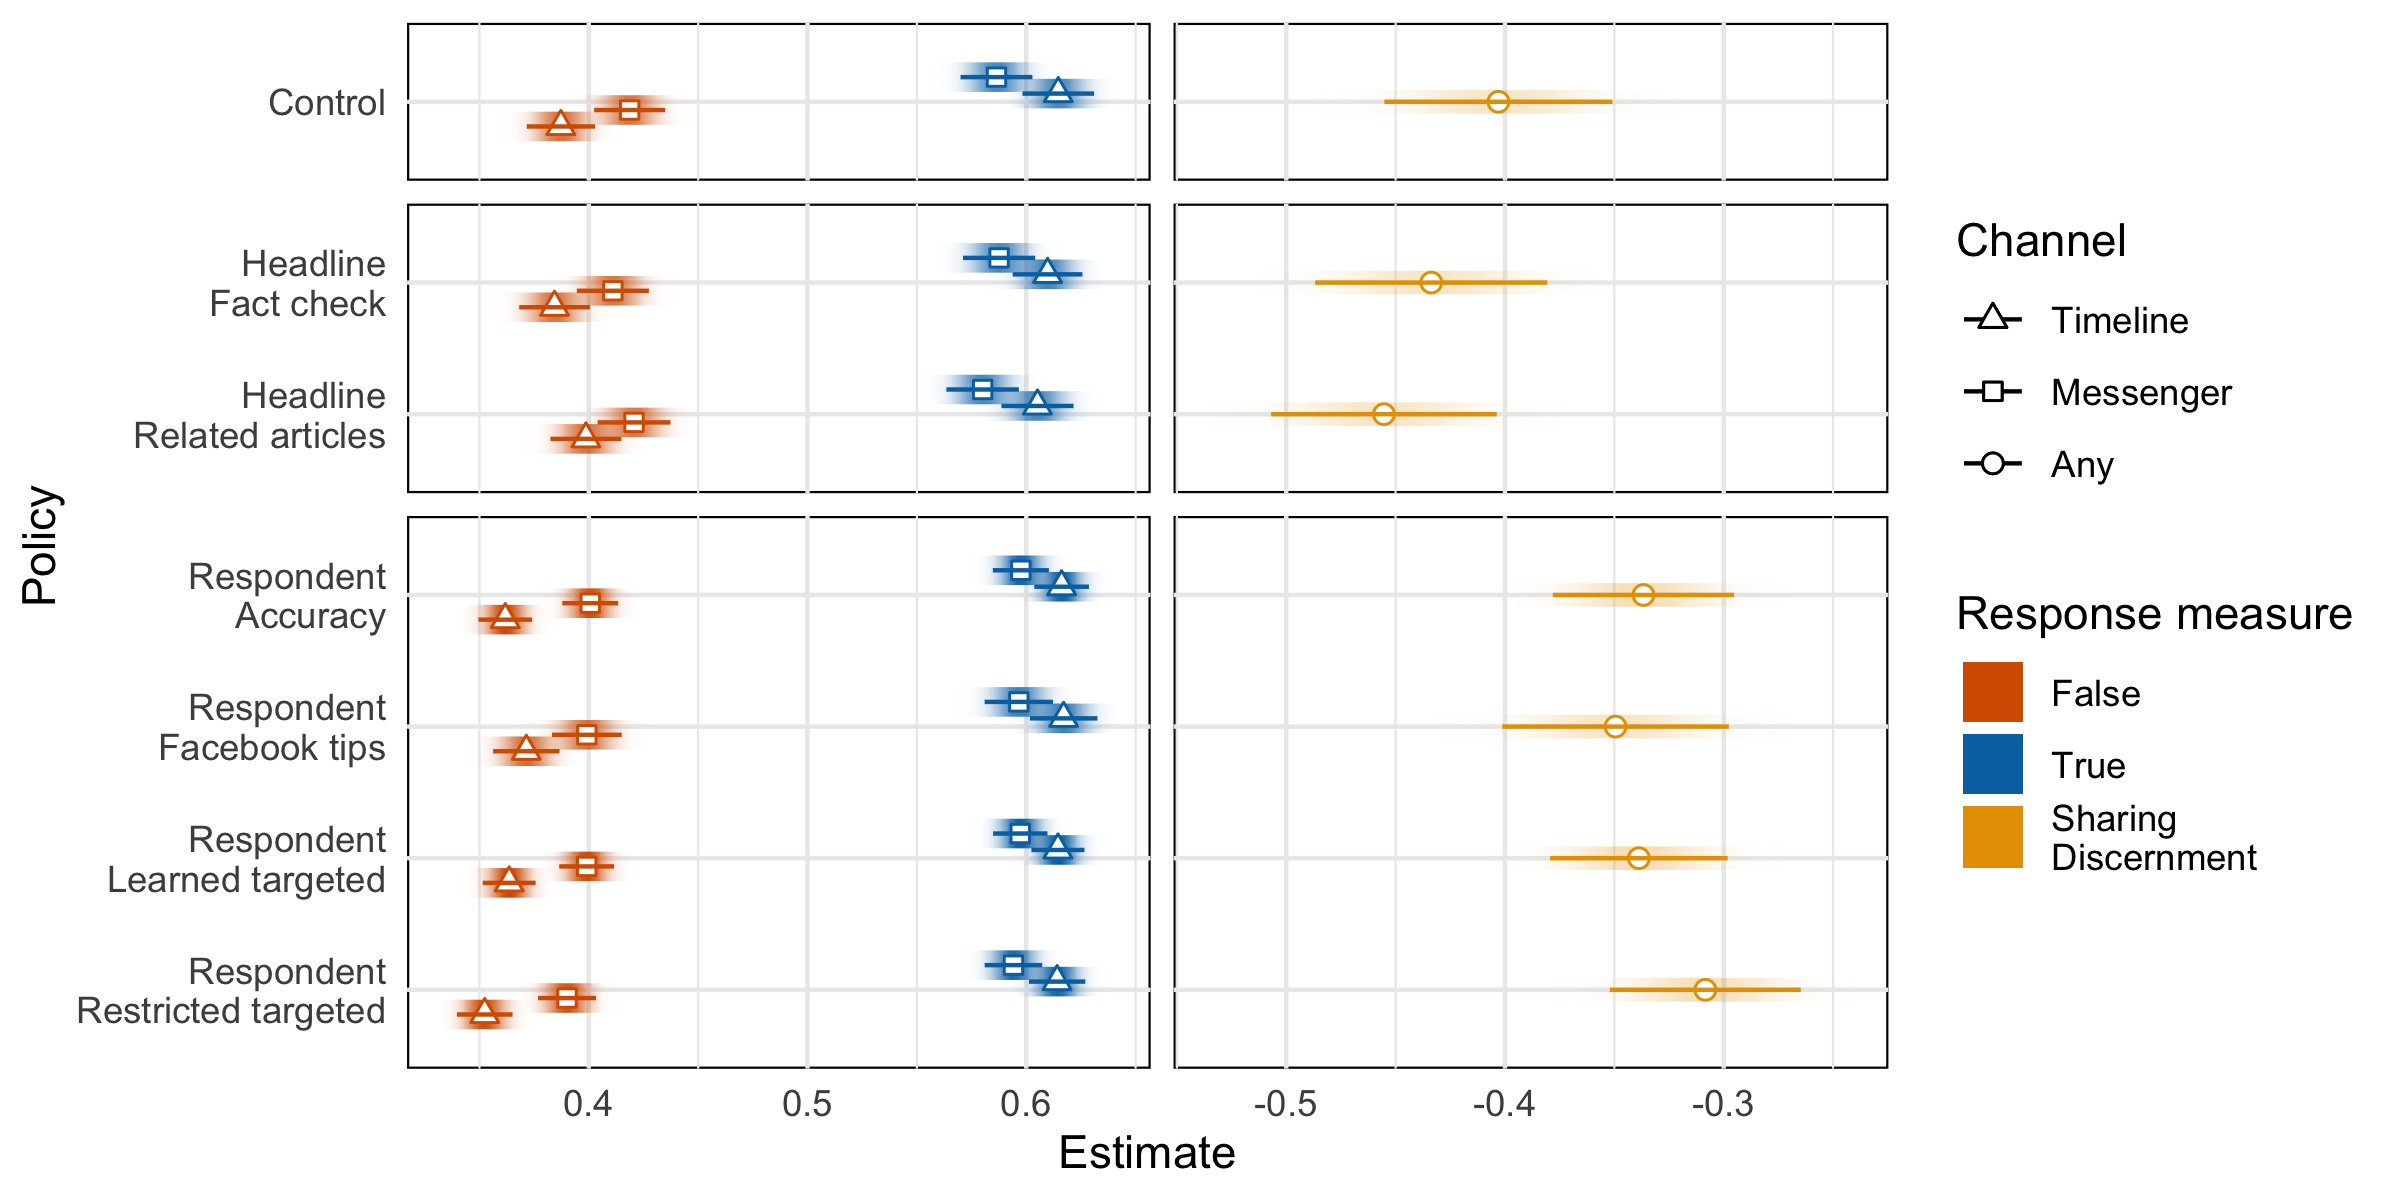
\includegraphics[width = \textwidth]{../analysis/figures/evaluated_scores_all.png}
\caption{\textbf{Response estimates.} Response measures are average intention to share true and false stimuli over either channel, and a combined response measure, reported in Section~\ref{section:measures}. Estimates are produced from an augmented inverse probability weighted estimator, as described in Section~\ref{section:estimation}.}
\label{fig:main_results}
\end{figure}
\todo{Alternative figure for main results}

Under control, we see that respondents exhibit discernment in what types of stimuli they share and over which channels. Respondents report greater intentions to share true stimuli as compared to false stimuli on any channel, and are more likely to share true stimuli on their public timelines as compared to by private message, but the reverse is true for false stimuli. This discernment by channel demonstrates that even when users intend to share false stimuli, they are making different decisions about the way in which they share it. 

We pre-specified tests of each type of treatment condition against the control. The two headline-level treatments are not effective towards our objective of decreasing sharing of false stimuli while maintaining rates of sharing true stimuli. The related articles treatment directionally increases intention to share false stimuli as compared to control, although this estimate is not statistically distinguishable from zero at conventional significance levels. The factcheck treatment is associated with a decrease of 0.5 pp (SE = 1.2)  as compared to control; the effect would need to be nearly four times as large with the same degree of uncertainty for the confidence interval to exclude zero. 

The respondent-level treatments, however, are more promising. The Facebook tips and accuracy nudge treatments decrease false sharing relative to control by 2.0 pp (SE = 1.0) and 3.3 pp (SE = 1.1), respectively, with small effects on true sharing, which are not distinguishable from zero at conventional significance levels. While both treatments are effective at decreasing public timeline sharing, the Facebook tips intervention is directionally more effective at also moving private sharing.\todo{Statement of effect size and significance here? Significance on difference in treatment effects across channels is marginal. } 

Other studies have found similar positive effects of accuracy prompts in diverse settings, including among quota-matched samples in 16 countries \citep{arechar2022understanding} and in a meta-analysis of 20 accuracy experiments with a total sample size over 20,000 \citep{pennycook2022accuracy}. Facebook tips have also been shown to be effective in the US and India \citep{guessetal2020digital}, indicating that both treatments may be scalable solutions for the global misinformation challenge. \citet{pennycook2021shifting} provide evidence that increased attention to the accuracy of articles is the mechanism driving the efficacy of the accuracy nudge. Previous research has not differentiated mechanisms driving the Facebook tips treatment, as both treatments appear to be effective for most participants. However, we find evidence of heterogeneity in treatment effects between the two treatments, suggesting that there are some differences in how these treatments work. 

To guard against experimenter demand effects, we embedded treatments in a longer survey block about general social media usage. If users' post-treatment response were, however, most responsive based on perceptions of what researchers want, we would expect the headline level treatments to have the largest decreases in false sharing intentions. For these treatments, only false stimuli were accompanied by visual flags. We do not find significant effects here, however. The variation in treatment effects by channel also provides evidence against experimenter demand effects: if users were only responding to perceived experimenter objectives, we would expect effects to be uniform across channels. %\todo{add more about variation in treatment effects by channel}


\subsection{Heterogeneous response and treatment effects}

We find covariates are highly predictive of heterogeneity in baseline sharing behaviors. In particular, we focus on several key variables for examining targeting and heterogeneity: age, gender, political allegiance, digital literacy, and scientific knowledge. We focus on these pre-registered variables as they may already be measured by social media platforms (age, gender) or of theoretical interest in social scientific research (political allegiance, digital literacy, and scientific knowledge).%
\footnote{%
Our digital literacy measure is an index of self-reported familiarity with computer and Internet-related terms adapted from \citet{guessmunger2020}.
Trust in science has been found to be a particularly strong predictor of belief in COVID misinformation/conspiracy theories \citep{murphy2021psychological}.
}

Policymakers with constrained resources may wish to better understand who to target to achieve maximum effect. Hence, it is worth understanding how targeting can be most effectively implemented. One approach to targeting is to identify the greatest culprits of sharing misinformation and direct interventions towards these users. Our data suggest that under control, younger participants, men, participants with low digital literacy, participants aligned with the ruling party, and participants with low scientific knowledge exhibit a higher propensity to share false stimuli (see Table~\ref{tab:heterogeneity_control}).

\begin{table}[H]
   \centering
\resizebox{!}{.325\paperheight}{ 
\begin{tabular}{lcccccc}
& \multicolumn{3}{c}{\textbf{False}} & \multicolumn{3}{c}{\textbf{True}} \\
& Any sharing & Messenger & Timeline & Any sharing & Messenger & Timeline \\
\cmidrule(lr){2-4}  \cmidrule(lr){5-7}
\multicolumn{4}{l}{\textbf{Age}} \rule{0pt}{1.2\normalbaselineskip} \\
\hspace{1em} Below median  & \num{0.457} & \num{0.413} & \num{0.375} & \num{0.633} & \num{0.547} & \num{0.563}\\
\hspace{1.5em} (n = 5,412) & (\num{0.012}) & (\num{0.012}) & (\num{0.011}) & (\num{0.012}) & (\num{0.012}) & (\num{0.012})\\
\hspace{1em} Above median & \num{0.425} & \num{0.376} & \num{0.363} & \num{0.671} & \num{0.575} & \num{0.623}\\
\hspace{1.5em} (n = 5,271)  & (\num{0.012}) & (\num{0.012}) & (\num{0.012}) & (\num{0.012}) & (\num{0.012}) & (\num{0.012})\\
\cmidrule(lr){2-7}
\hspace{1em} Difference& \num{0.032}+ & \num{0.038}* & \num{0.012} & \num{-0.038}* & \num{-0.028} & \num{-0.060}***\\
 & (\num{0.018}) & (\num{0.017}) & (\num{0.016}) & (\num{0.017}) & (\num{0.018}) & (\num{0.017})\\
 \multicolumn{4}{l}{\textbf{Gender}}  \rule{0pt}{1.2\normalbaselineskip}\\
\hspace{1em} Not male   & \num{0.400} & \num{0.359} & \num{0.327} & \num{0.611} & \num{0.512} & \num{0.543}\\
\hspace{1.5em}  (n = 5,050)& (\num{0.012}) & (\num{0.012}) & (\num{0.011}) & (\num{0.012}) & (\num{0.013}) & (\num{0.012})\\
\hspace{1em} Male & \num{0.479} & \num{0.426} & \num{0.407} & \num{0.687} & \num{0.604} & \num{0.638}\\
 \hspace{1.5em}  (n = 5,633)  & (\num{0.012}) & (\num{0.012}) & (\num{0.012}) & (\num{0.011}) & (\num{0.012}) & (\num{0.012})\\
\cmidrule(lr){2-7}
\hspace{1em} Difference  & \num{-0.078}*** & \num{-0.078}*** & \num{-0.078}*** & \num{-0.076}*** & \num{-0.076}*** & \num{-0.076}***\\
 & (\num{0.018}) & (\num{0.018}) & (\num{0.018}) & (\num{0.017}) & (\num{0.017}) & (\num{0.017})\\
 \multicolumn{4}{l}{\textbf{Political allegiance}} \rule{0pt}{1.2\normalbaselineskip}\\
\hspace{1em} Not aligned & \num{0.416} & \num{0.365} & \num{0.341} & \num{0.630} & \num{0.535} & \num{0.564}\\
\hspace{1.5em} (n = 7,570)  & (\num{0.010}) & (\num{0.010}) & (\num{0.010}) & (\num{0.010}) & (\num{0.010}) & (\num{0.010})\\\hspace{1em} Aligned  (n = 3113) & \num{0.505} & \num{0.467} & \num{0.438} & \num{0.704} & \num{0.622} & \num{0.662}\\
 & (\num{0.016}) & (\num{0.016}) & (\num{0.015}) & (\num{0.015}) & (\num{0.016}) & (\num{0.016})\\
 \cmidrule(lr){2-7}
\hspace{1em} Difference & \num{-0.090}*** & \num{-0.090}*** & \num{-0.090}*** & \num{-0.074}*** & \num{-0.074}*** & \num{-0.074}***\\
 & (\num{0.019}) & (\num{0.019}) & (\num{0.019}) & (\num{0.018}) & (\num{0.018}) & (\num{0.018})\\
\multicolumn{4}{l}{\textbf{Digital literacy index }}  \rule{0pt}{1.2\normalbaselineskip}\\
\hspace{1em} Below median & \num{0.495} & \num{0.448} & \num{0.423} & \num{0.675} & \num{0.587} & \num{0.621}\\
 \hspace{1.5em}  (n = 5,443) & (\num{0.012}) & (\num{0.012}) & (\num{0.012}) & (\num{0.011}) & (\num{0.012}) & (\num{0.012})\\\hspace{1em} Above median  & \num{0.387} & \num{0.340} & \num{0.314} & \num{0.627} & \num{0.533} & \num{0.564}\\
 \hspace{1.5em}  (n = 5,240) & (\num{0.012}) & (\num{0.012}) & (\num{0.011}) & (\num{0.012}) & (\num{0.013}) & (\num{0.013})\\
\cmidrule(lr){2-7}
\hspace{1em} Difference & \num{0.108}*** & \num{0.108}*** & \num{0.109}*** & \num{0.048}** & \num{0.055}** & \num{0.058}***\\
 & (\num{0.018}) & (\num{0.017}) & (\num{0.016}) & (\num{0.017}) & (\num{0.018}) & (\num{0.017})\\
\multicolumn{4}{l}{\textbf{Scientific knowledge index}} \rule{0pt}{1.2\normalbaselineskip} \\
\hspace{1em} Below median & \num{0.459} & \num{0.412} & \num{0.384} & \num{0.659} & \num{0.561} & \num{0.597}\\
 \hspace{1.5em}   (n = 5,677) & (\num{0.012}) & (\num{0.012}) & (\num{0.011}) & (\num{0.012}) & (\num{0.012}) & (\num{0.012})\\
 \hspace{1em} Above median& \num{0.423} & \num{0.375} & \num{0.352} & \num{0.643} & \num{0.560} & \num{0.588}\\
 \hspace{1.5em}  (n = 5,006)  & (\num{0.013}) & (\num{0.012}) & (\num{0.012}) & (\num{0.012}) & (\num{0.013}) & (\num{0.013})\\\cmidrule(lr){2-7}
\hspace{1em} Difference  & \num{0.036}* & \num{0.036}* & \num{0.031}+ & \num{0.016} & \num{0.002} & \num{0.010}\\
 & (\num{0.018}) & (\num{0.017}) & (\num{0.016}) & (\num{0.017}) & (\num{0.018}) & (\num{0.017})\\
   \end{tabular}}
   \caption{\textbf{Heterogeneity in response under the control condition by selected covariates.} Estimates are of mean response under the control condition, and are produced from an augmented inverse probability weighted estimator, as described in Section~\ref{section:estimation}, within specified subgroups. For differences only: \textsuperscript{+} $p<0.1$, \textsuperscript{*} $p < 0.05$, \textsuperscript{**} $p < 0.01$, \textsuperscript{***} $p < 0.001$.}   
   \label{tab:heterogeneity_control}
\end{table}


For these groups we find that assigning either the accuracy nudge or the Facebook tips treatment on average decreases false sharing as compared to control among participants with low digital literacy (-4.3, SE = 1.4), men (-3.3, SE = 1.3), and participants with low scientific knowledge (-4.5, SE =1.3). (See Table~\ref{tab:heterogeneity_treatment}.) The pooled respondent-level interventions do not reduce sharing of false posts among younger participants but do among older ones. Similarly, there is no effect of the pooled respondent treatments on false sharing among those aligned with the political party in power but we do see a significant effect among those not aligned. However, \textit{differences} in treatment effects across groups are only statistically significant when comparing users with low to those with high levels of scientific knowledge.

\textcolor{red}{[TK: comments about heterogeneity in channel sharing.]} 

\begin{table}[H]
\small
   \centering
\resizebox{!}{.325\paperheight}{ 
\begin{tabular}{lcccccc}
& \multicolumn{3}{c}{\textbf{False}} & \multicolumn{3}{c}{\textbf{True}} \\
& Any sharing & Messenger & Timeline & Any sharing & Messenger & Timeline \\
\cmidrule(lr){2-4}  \cmidrule(lr){5-7}
\multicolumn{4}{l}{\textbf{Age}} \rule{0pt}{1.2\normalbaselineskip} \\
\hspace{1em} Below median  & \num{-0.018} & \num{-0.021} & \num{-0.018} & \num{-0.025}+ & \num{-0.019} & \num{-0.035}*\\
\hspace{1.5em} (n = 5,412)& (\num{0.014}) & (\num{0.013}) & (\num{0.012}) & (\num{0.014}) & (\num{0.014}) & (\num{0.014})\\
\hspace{1em} Above median  & \num{-0.035}* & \num{-0.026}+ & \num{-0.038}** & \num{0.009} & \num{0.019} & \num{0.002}\\
 \hspace{1.5em} (n = 5,271) & (\num{0.014}) & (\num{0.013}) & (\num{0.013}) & (\num{0.013}) & (\num{0.014}) & (\num{0.014})\\
  & (0.014) & (0.013) & (0.013) & (0.013) & (0.014) & (0.014) \\
\cmidrule(lr){2-7}
 \hspace{1em} Difference & \num{0.016} & \num{0.005} & \num{0.021} & \num{-0.034}+ & \num{-0.038}+ & \num{-0.037}+\\
 & (\num{0.019}) & (\num{0.018}) & (\num{0.018}) & (\num{0.019}) & (\num{0.019}) & (\num{0.019})\\
  \multicolumn{4}{l}{\textbf{Gender}}  \rule{0pt}{1.2\normalbaselineskip}\\
\hspace{1em}Not male& \num{-0.019} & \num{-0.022}+ & \num{-0.021}+ & \num{-0.024}+ & \num{-0.004} & \num{-0.029}*\\
\hspace{1.5em} (n = 5,050) & (\num{0.014}) & (\num{0.013}) & (\num{0.012}) & (\num{0.014}) & (\num{0.014}) & (\num{0.014})\\
\hspace{1em} Male  & \num{-0.033}* & \num{-0.024}+ & \num{-0.034}** & \num{0.006} & \num{0.004} & \num{-0.005}\\
\hspace{1.5em}  (n = 5,633)& (\num{0.013}) & (\num{0.013}) & (\num{0.013}) & (\num{0.013}) & (\num{0.013}) & (\num{0.013})\\
 \cmidrule(lr){2-7}
 \hspace{1em} Difference & \num{0.014} & \num{0.002} & \num{0.013} & \num{-0.030} & \num{-0.007} & \num{-0.025}\\
\hspace{1.5em} & (\num{0.019}) & (\num{0.018}) & (\num{0.018}) & (\num{0.019}) & (\num{0.019}) & (\num{0.019})\\
  \multicolumn{4}{l}{\textbf{Political allegiance}} \rule{0pt}{1.2\normalbaselineskip}\\
\hspace{1em} Not aligned  & \num{-0.035}** & \num{-0.029}** & \num{-0.040}*** & \num{-0.007} & \num{0.004} & \num{-0.015}\\
\hspace{1.5em} (n = 7,570) & (\num{0.011}) & (\num{0.011}) & (\num{0.011}) & (\num{0.011}) & (\num{0.012}) & (\num{0.012})\\
\hspace{1em} Aligned  & \num{-0.006} & \num{-0.009} & \num{0.001} & \num{-0.012} & \num{-0.009} & \num{-0.019}\\
\hspace{1.5em} (n = 3,113)& (\num{0.018}) & (\num{0.017}) & (\num{0.017}) & (\num{0.017}) & (\num{0.018}) & (\num{0.017})\\
  \cmidrule(lr){2-7}
 \hspace{1em} Difference & \num{-0.029} & \num{-0.020} & \num{-0.041}* & \num{0.005} & \num{0.012} & \num{0.004}\\
\hspace{1.5em} & (\num{0.021}) & (\num{0.020}) & (\num{0.020}) & (\num{0.021}) & (\num{0.021}) & (\num{0.021})\\
 \multicolumn{4}{l}{\textbf{Digital literacy index }}  \rule{0pt}{1.2\normalbaselineskip}\\
\hspace{1em} Below median & \num{-0.043}** & \num{-0.039}** & \num{-0.038}** & \num{-0.025}+ & \num{-0.012} & \num{-0.025}+\\
\hspace{1.5em}  (n = 5,443)& (\num{0.014}) & (\num{0.013}) & (\num{0.013}) & (\num{0.013}) & (\num{0.013}) & (\num{0.013})\\
\hspace{1em} Above median & \num{-0.009} & \num{-0.007} & \num{-0.018} & \num{0.008} & \num{0.012} & \num{-0.007}\\
\hspace{1.5em} (n = 5,240)  & (\num{0.014}) & (\num{0.013}) & (\num{0.012}) & (\num{0.014}) & (\num{0.014}) & (\num{0.014})\\
 \cmidrule(lr){2-7}
\hspace{1em} Difference & \num{-0.033}+ & \num{-0.032}+ & \num{-0.020} & \num{-0.033}+ & \num{-0.024} & \num{-0.018}\\
 & (\num{0.019}) & (\num{0.018}) & (\num{0.018}) & (\num{0.019}) & (\num{0.019}) & (\num{0.019})\\
 \multicolumn{4}{l}{\textbf{Scientific knowledge index }}  \rule{0pt}{1.2\normalbaselineskip}\\
\hspace{1em}   Below median  & \num{-0.045}*** & \num{-0.044}*** & \num{-0.040}** & \num{-0.026}* & \num{-0.011} & \num{-0.033}*\\
\hspace{1.5em} (n = 5,677)& (\num{0.013}) & (\num{0.013}) & (\num{0.012}) & (\num{0.013}) & (\num{0.014}) & (\num{0.013})\\
\hspace{1em}   Above median& \num{-0.006} & \num{0.001} & \num{-0.014} & \num{0.012} & \num{0.013} & \num{0.002}\\
\hspace{1.5em}  (n = 5,006) & (\num{0.014}) & (\num{0.013}) & (\num{0.013}) & (\num{0.013}) & (\num{0.014}) & (\num{0.014})\\
 \cmidrule(lr){2-7}
\hspace{1em}   Difference & \num{-0.039}* & \num{-0.045}* & \num{-0.026} & \num{-0.038}* & \num{-0.024} & \num{-0.035}+\\
 & (\num{0.019}) & (\num{0.018}) & (\num{0.018}) & (\num{0.019}) & (\num{0.019}) & (\num{0.019})\\
    \end{tabular}
   }
   \caption{\textbf{Heterogeneity in treatment effects under averaged respondent-level treatments by selected covariates.} Estimates are of treatment effects averaged across the two respondent-level treatments, in contrast with the control condition. Estimates are produced from an augmented inverse probability weighted estimator, as described in Section~\ref{section:estimation}, within specified subgroups. \textsuperscript{+} $p<0.1$, \textsuperscript{*} $p < 0.05$, \textsuperscript{**} $p < 0.01$, \textsuperscript{***} $p < 0.001$.}
  \label{tab:heterogeneity_treatment}
\end{table}\todo{Note that this table represents \textbf{treatment effect estimates} in comparison to control, whereas Table 2 represents control mean. Is this confusing? Better way to differentiate?}
\todo{replicate table with treatment effects as percent change over baseline}

\begin{figure}[H]
\includegraphics[width = \textwidth]{../analysis/figures/any_sharing_by_covariates_te_comparisons_false.png}
\caption{Response under the control condition. The outcome measure is the proportion of true or false stimuli participants reported wanting to share, either as a Facebook post or privately in Facebook Messenger. Estimates are produced from an augmented inverse probability weighted estimator, as described in Section~\ref{section:estimation}, within specified subgroups.}
\label{fig:treatments}
\end{figure}\todo{Alternative figure}


\subsection{Heterogeneity in best policy}\label{section:het_policy}

We can also consider targeting in terms of which participants should get which treatment. We estimate average decreases in false sharing intentions for both the accuracy nudge and the Facebook tips treatment. However, we also observe differences in how users respond to these two treatments. Figure~\ref{fig:RATE} shows differences in average response under the accuracy nudge as compared to Facebook tips, if we were to assign the accuracy nudge according to a prioritization rule instead of at random, following the approach presented in \citet{yadlowsky2021evaluating}. Here the prioritization rule is assigned by fitting a causal forest on the learning data, predicting response under the model on the evaluation data, and ordering based on predicted differences. We can see, for example, that if we were limited to assigning the accuracy nudge to only 40 percent of the population, false sharing intentions would be 4.4 pp lower (SE = 1.5) if we used the prioritization rule instead of random assignment. The overall rank-weighted average treatment effect, a weighted sum of the area under the curve in Figure~\ref{fig:RATE}, is -3.8 pp (SE = 1.3), using the targeting operator characteristic curve. 

\begin{figure}[H] %  figure placement: here, top, bottom, or page
   \centering
   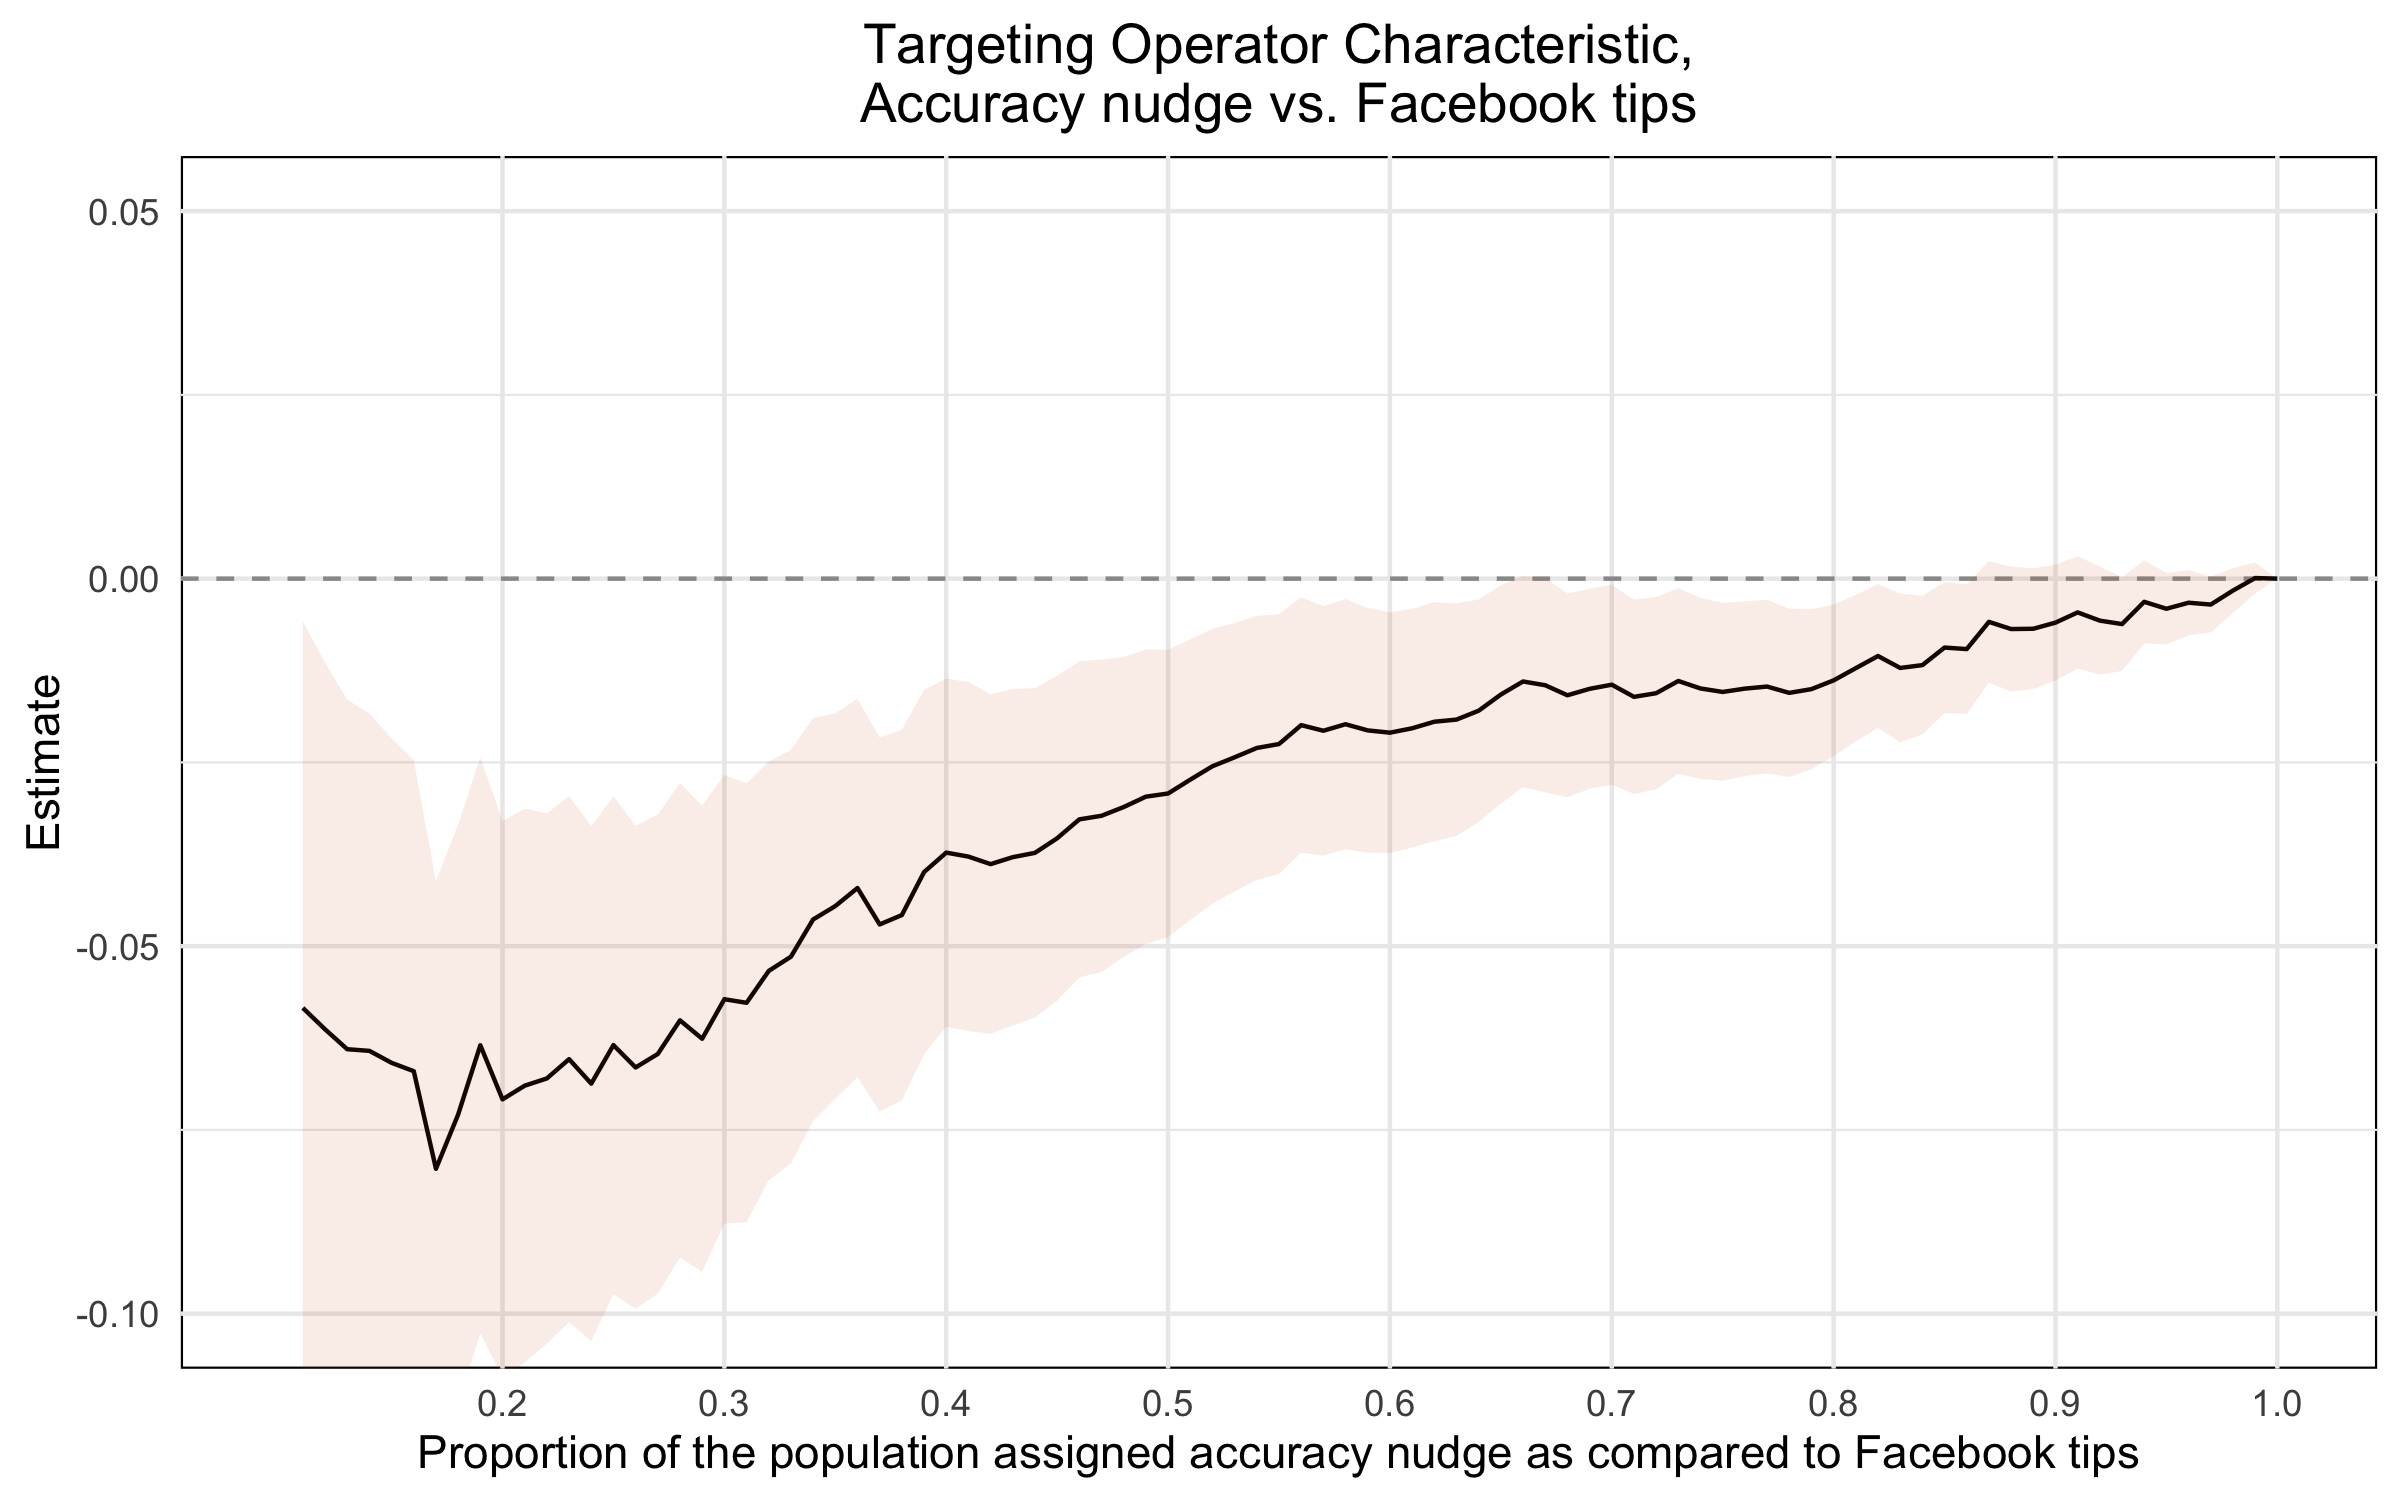
\includegraphics[width=\textwidth]{../analysis/figures/rate_accuracy_vs_facebook.png} 
   \caption{\textbf{Targeting operator characteristic curve, comparing the accuracy nudge and Facebook tips.} The outcome measure is the difference in proportion of false stimuli participants reported wanting to share, either as a Facebook post or privately in Facebook Messenger, between the accuracy nudge and Facebook tips. The y-axis represents differences in this measure if the users receiving the accuracy nudge were assigned according to a prioritization rule, as compared to at random. The shaded region shows the 95\% confidence interval.}
   \label{fig:RATE}
\end{figure}

To evaluate the overall effect of targeting, we consider the causal forest model learned for prioritization rule above as a contextual policy: if the predicted difference difference between the accuracy nudge and the Facebook tips treatment is negative (indicating that the accuracy nudge is more effective at decreasing false sharing), our policy assigns the accuracy nudge; otherwise the Facebook tips treatment is assigned.  

When the model is applied to the evaluation data, our optimal contextual policy assigns 43.5\% of participants to Facebook tips, which is the best uniform policy for decreasing sharing of false stimuli. The 46.5\% of participants assigned to the accuracy nudge are, on average, more digitally literate, more likely to have more scientific knowledge,
more likely to be male, older, and directionally more likely to be aligned with the governing political party (see Figure~\ref{fig:heterogeneity_covariates}).

\begin{figure}[H] %  figure placement: here, top, bottom, or page
   \centering
   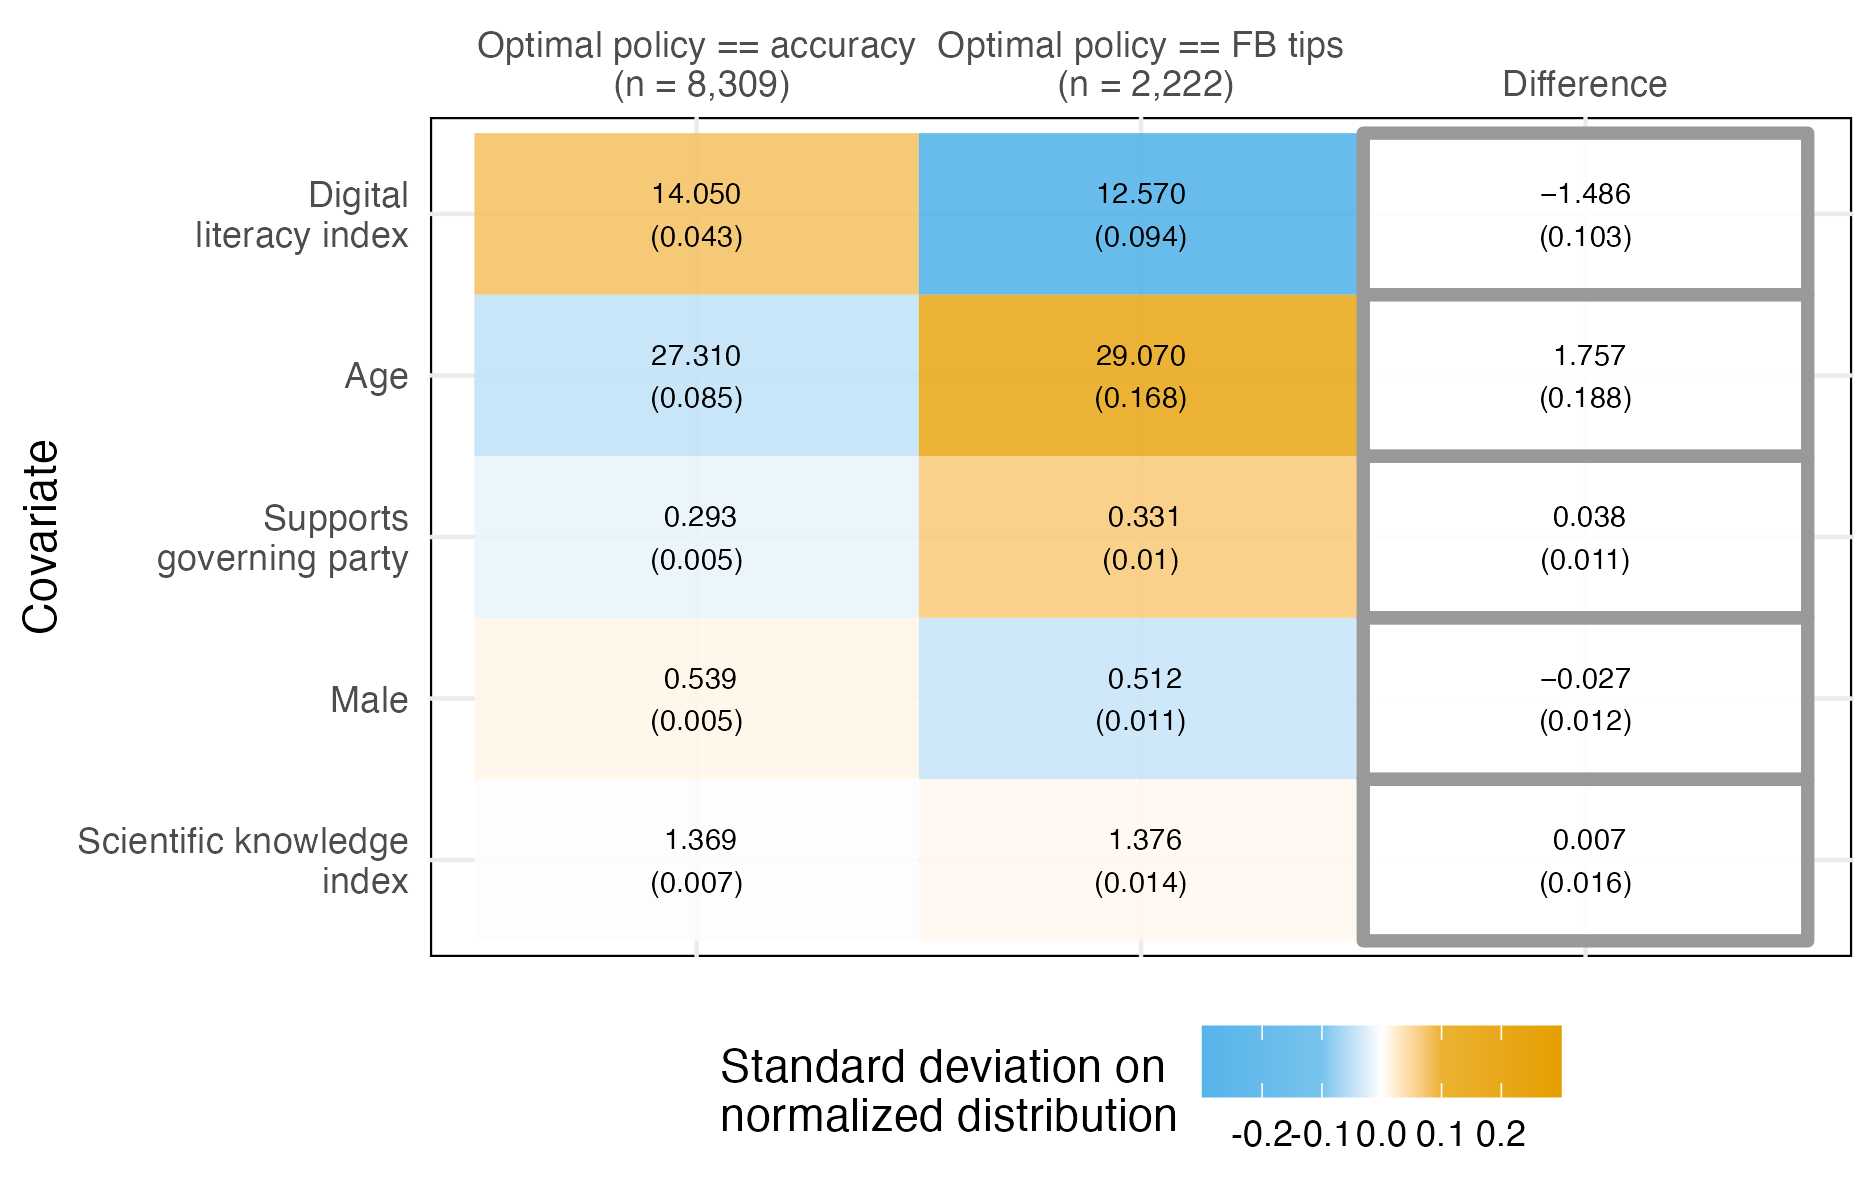
\includegraphics[width=\textwidth]{../analysis/figures/covariate_optimal.png} 
   \caption{\textbf{Selected covariate means between participants assigned to the accuracy nudge as compared to participants assigned to Facebook tips under the contextual policy.} Covariates are ordered by size of standardized deviation between the two groups. }
   \label{fig:heterogeneity_covariates}
\end{figure}\todo{Should this figure just be a table?}

Optimally assigning these treatments, we achieve a treatment effect of -3.9 percentage points (SE = 1.1) in decreasing false sharing intentions.  We saw in Table~\ref{tab:main_results} that we achieve larger magnitude treatment effects in decreasing false sharing intentions through our contextual policy as compared to either the accuracy nudge or the Facebook tips treatments assigned uniformly (one-sided p-values for difference of 0.002 and 0.130, respectively).  

In Table~\ref{tab:heterogeneity_best}, we see that our contextual policy learned on the learning data is appropriately assigning participants to the respective respondent-level conditions: participants for whom assignment under the learned optimal policy is Facebook tips on average intend to share false information at lower rates under the Facebook tips treatment as compared to the accuracy nudge (difference of 3.8, SE = 1.4); the reverse is true directionally for the participants assigned the accuracy nudge under the learned optimal policy (difference of -1.7, SE = 1.5).  The heterogeneity in treatment effects between the two groups (difference of 3.8, SE = 1.4) provides new evidence that participants respond differently to these two treatments. 


\begin{table}[H]
\small
   \centering
%\resizebox{\textwidth}{!}{ 
\begin{tabular}{lcccccc}
& \multicolumn{3}{c}{\textbf{False}} & \multicolumn{3}{c}{\textbf{True}} \\
& Any sharing & Messenger & Timeline & Any sharing & Messenger & Timeline \\
\cmidrule(lr){2-4}  \cmidrule(lr){5-7}
\multicolumn{4}{l}{\textbf{Optimal assignment == Accuracy nudge} (n = 4,967)} \rule{0pt}{1.2\normalbaselineskip} \\
\hspace{1em} Accuracy & \num{0.396} & \num{0.349} & \num{0.341} & \num{0.681} & \num{0.588} & \num{0.637}\\
 & (\num{0.010}) & (\num{0.009}) & (\num{0.009}) & (\num{0.010}) & (\num{0.010}) & (\num{0.010})\\
\hspace{1em} Facebook tips & \num{0.412} & \num{0.363} & \num{0.352} & \num{0.687} & \num{0.602} & \num{0.639}\\
 & (\num{0.012}) & (\num{0.012}) & (\num{0.011}) & (\num{0.013}) & (\num{0.013}) & (\num{0.013})\\
   \cmidrule(lr){2-7}
 \hspace{1em} Difference & \num{-0.016} & \num{-0.014} & \num{-0.012} & \num{-0.006} & \num{-0.014} & \num{-0.001}\\
 & (\num{0.015}) & (\num{0.015}) & (\num{0.015}) & (\num{0.016}) & (\num{0.016}) & (\num{0.016})\\
\multicolumn{4}{l}{\textbf{Optimal assignment == Facebook tips} (n = 5,716)} \rule{0pt}{1.2\normalbaselineskip} \\
\hspace{1em} Accuracy & \num{0.445} & \num{0.401} & \num{0.345} & \num{0.622} & \num{0.547} & \num{0.534}\\
 & (\num{0.009}) & (\num{0.009}) & (\num{0.009}) & (\num{0.009}) & (\num{0.009}) & (\num{0.009})\\
\hspace{1em} Facebook tips & \num{0.407} & \num{0.367} & \num{0.330} & \num{0.589} & \num{0.516} & \num{0.513}\\
 & (\num{0.011}) & (\num{0.011}) & (\num{0.011}) & (\num{0.011}) & (\num{0.011}) & (\num{0.011})\\
   \cmidrule(lr){2-7}
 \hspace{1em} Difference & \num{0.038}** & \num{0.034}* & \num{0.014} & \num{0.033}* & \num{0.031}* & \num{0.021}\\
 & (\num{0.014}) & (\num{0.014}) & (\num{0.014}) & (\num{0.015}) & (\num{0.015}) & (\num{0.015})\\
\hline
\multicolumn{4}{l}{\textbf{Grand difference}} \rule{0pt}{1.2\normalbaselineskip} \\
  \num{0.054}* & \num{0.048}* & \num{0.026} & \num{0.039}+ & \num{0.045}* & \num{0.023}\\
 & (\num{0.021}) & (\num{0.021}) & (\num{0.020}) & (\num{0.022}) & (\num{0.022}) & (\num{0.021})\\
   \end{tabular}
%   }
   \caption{\textbf{Response under counterfactual uniform respondent treatment conditions, by contextual policy assignment.} Estimates are of mean response under the two respondent-level treatments. Estimates are produced from an augmented inverse probability weighted estimator, as described in Section~\ref{section:estimation}, within specified subgroups. For differences only: \textsuperscript{+} $p<0.1$, \textsuperscript{*} $p < 0.05$, \textsuperscript{**} $p < 0.01$, \textsuperscript{***} $p < 0.001$.}
   \label{tab:heterogeneity_best}
\end{table}


%\begin{figure}[H]
%\centering
%\includegraphics[width = \textwidth]{../analysis/figures/r_accuracy_scores_any_false_r_tips_facebook_scores_any_false_optimal_assignment.png}
%   \caption{\textbf{Response under counterfactual uniform respondent treatment conditions, by contextual policy assignment.} Estimates are produced from an augmented inverse probability weighted estimator, as described in Section~\ref{section:estimation}, within specified subgroups.}
%   \label{fig:heterogeneity_best}
%\end{figure}


%%%%%%%%%%%%%%%%%%%%%%%%%%%%%%%%%%%%%%%%%%%%
%DISCUSSION
%%%%%%%%%%%%%%%%%%%%%%%%%%%%%%%%%%%%%%%%%%%%


\section{Discussion}

This study, like others of its kind, has limitations. Importantly, the data come from a survey experiment, rather than a field experiment. However, the design of the study offers enhanced realism for participants beyond the standard approach of recruitment of samples through survey firms, and implementation of surveys on web browser-based platforms. Instead, we recruit social media users on the Facebook platform itself, where they would normally come into contact with online (mis)information about COVID-19. We keep participants on the platform interacting with a Messenger bot, which may feel somewhat more naturalistic than answering survey questions using another software, but is still an experimenter-controlled environment. This control facilitated more straightforward measurement, and also reduces ethical concerns about the possibility of the experiment facilitating the spread of COVID misinformation during a global pandemic. 

Acknowledging these limitations, we believe this study offers insights useful for fighting online misinformation globally. The key insight is that low-cost and scalable accuracy nudges and tips for spotting misinformation delivered to users as they scroll social media can be effective in many diverse contexts. This study provides evidence that such interventions are more effective than many others often tested by academics and used by platforms. Platforms may be more likely to deliver such interventions knowing that they help reduce sharing of misinformation without harming sharing of true information. Such policies delivered to participants are much more cost effective than headline-specific interventions that require time and effort from human or AI fact checkers.

Ours is one of only a few studies examining Facebook's related articles policy \citep[see also][]{bode2015related}, hence more research is needed. The fact that we do not see effects from fact-checking interventions in this setting may raise concerns given the existing evidence of disputed labels and warnings from the US and other high-income countries. However, we believe that these results may vary across settings given the variations in context, specifically the general levels of digital literacy and abilities to discern fact from fiction. For instance, when we analyze the headline-level interventions by baseline-levels of sharing ``discernment'' (pre-treatment sharing of true $>$ false information), we find that there is a group of participants for whom showing related articles under false posts reduces false sharing compared to control. 

Specifically, participants with pretreatment sharing discernment above the sample median share false news less under related articles treatment as compared to control ($p < 0.05$), participants below median share false news more under related articles ($p < 0.06$), and the difference is significant at $p < 0.01$. Participants with above median baseline levels of sharing discernment share false stimuli (along either channel) 19.1 percent of the time. Under the related articles treatment, this sharing is decreased by 1.4 pp, a 7.2 percent reduction. These findings perhaps hint at the idea that more ambiguous post-level interventions such as showing related articles are only effective among already well-discerning individuals. This may also help to explain our general finding of no effects from headline-level treatments among our sample---who may have lower baseline discernment than samples from high-income countries that may have generally higher levels of education or have greater digital literacy. More research from diverse contexts is required to understand which interventions are effective and why some treatments that work in certain settings are not effective in others.

\section{Acknowledgements}
\textcolor{red}{[TK: Facebook Health; James, Ricardo, Undral; feedback from various workshops.]}

%%%%%%%%%%%%%%%%%%%%%%%%%%%%%%%%%%%%%%%%%%%%
%BIBLIOGRAPY
%%%%%%%%%%%%%%%%%%%%%%%%%%%%%%%%%%%%%%%%%%%%

\bibliography{../preanalysis/fb_misinfo_references.bib}

\clearpage


%%%%%%%%%%%%%%%%%%%%%%%%%%%%%%%%%%%%%%%%%%%%
%APPENDIX
%%%%%%%%%%%%%%%%%%%%%%%%%%%%%%%%%%%%%%%%%%%%


\appendix
\phantomsection\label{SI}
\renewcommand\thefigure{S\arabic{figure}} 
\renewcommand\thetable{S\arabic{table}} 
 \renewcommand{\thesection}{S\arabic{section}}
 \pagenumbering{arabic}
\renewcommand*{\thepage}{SI.\arabic{page}}
\setcounter{figure}{0} 
\setcounter{table}{0} 
\appendixpage


  \startcontents
  \printcontents{}{1}{}
  
 \clearpage
  
\section{Design and measurement}

\subsection{Recruitment}
We conduct this study with social media users in two major English-language hubs of online communication in sub-Saharan Africa, Kenya and Nigeria. Facebook  estimates that there  are  30-35  million  Facebook  users  who  are 18 years and older from these two countries (as reported on the audience insights tool on Facebook's advertising platform).  AfricaCheck.org, a third party verification site, has offices in both countries and has recently created pages devoted to coronavirus-related misinformation circulating online. From January to March, the number of English-language ``fact-checks'' (i.e., publicly spread pieces of information deemed false or misleading by fact-checking organizations) increased by more than 900\% worldwide (Brennen et al.,2020), demonstrating the prevalence of this kind of content and the availability of verified COVID-related information. Both countries also have at some point had access to Facebook zero, a light free version of Facebook, meaning that users do not need to pay for data to access certain features of the platform. 

As is becoming increasingly popular among social scientists, we recruited social media users 18 years and over in Kenya and Nigeria through targeted Facebook advertisements \citep{Rosenzweig_2020}. Users who clicked on our ads offering airtime for taking a survey (see Figure~\ref{fig:recruitment}) then started a conversation with our page's Messenger chatbot. In contrast to sending users to an external survey platform such as Qualtrics, the benefit of the chatbot is that we keep users on the Facebook platform, with which they are likely more familiar, and maintain a realistic setting in which users might encounter online misinformation. Participants who completed the survey in the chatbot received compensation in the form of mobile phone airtime (equivalent to about \$0.50) sent to their phone.

\begin{figure}[H]
\centering
\includegraphics[width = 0.8\textwidth]{../analysis/figures/advertisement_2020-10-26.png}
   \caption{\textbf{Advertising image used for recruitment.}}
   \label{fig:recruitment}
\end{figure}

\subsection{Survey instrument}
The survey script is available at this link:\\
\url{http://bit.ly/facebook_survey_public}

All of the stimuli (posts) used in the experiment are available at this link:\\
\url{http://bit.ly/facebook_stimuli_public}

\subsection{Treatments}\label{appendix:treatments}

Treatments 1, 2, 3, 8, 9 and 10 are derived from interventions currently being used by social media platforms including Facebook, Twitter, and WhatsApp. For instance, Guess et al. (2020) find that reading Facebook's tips for spotting untrustworthy news improved participants' ability to discern false from true headlines in the US and India. Treatment 11 (real information) is a similar headline-level treatment that \textit{could} be adopted by industry partners. Rather than flags or warnings about misinformation, we test whether providing a simple true statement reduces sharing of false information. Existing research suggests that providing true information can sometimes influence individuals' attitudes and behaviors (Gilens, 2001). Treatments 4, 6, and 7 are taken from previous academic studies. The accuracy nudge treatment (6) was specifically found to be effective at reducing the sharing of COVID-19 misinformation among participants in the US. Our deliberation nudge treatment (7) was adapted from Bago et al. (2020) that found asking participants to deliberate to be effective at improving discernment of online political information. Emotions have been suspected to influence susceptibility to misinformation (Martel et al., 2019), our test evaluates one canonical method of emotion suppression as a way to reduce the influence of misinformation. The pledge treatment (5) was adapted from the types of treatments used by political campaigns to get subjects to pledge to vote or support a particular candidate (Costa et al., 2018). We vary whether the pledge is made in private (within the chatbot conversation) or in public (posted on the respondent's Facebook timeline) to test whether public pledges are more effective at influencing behavior than private ones (Cotterill et al., 2013). 

\begin{table}[H]
\centering
\resizebox{\textwidth}{!}{ 
\begin{tabular}{l|l|l}
\multicolumn{1}{l|}{\textbf{\begin{tabular}[c]{@{}c@{}}Shorthand\\ Name\end{tabular}}} & \multicolumn{1}{c|}{\textbf{\begin{tabular}[c]{@{}c@{}}Treatment\\ Level\end{tabular}}} & \textbf{Treatment}                                                                                                                                                                                                                                                                                                                                                                                              \\ \hline
1. Facebook tips                                                                                                           & Respondent                                                                                                   &  Facebook's ``Tips to Spot False News'' 
\\
2. AfricaCheck tips                                                                                                         & Respondent                                                                                                   &  \url{Africacheck.org}'s guide: \\ & & ``How to vet information during a pandemic''                                                                                                                                                                                                                                                                                                                             \\
3. Video training
 & Respondent                                                                                                   &   \href{https://www.facebook.com/Vodcasts/videos/1322816708106278/}{BBC video} on spotting Coronavirus misinformation %, \href{https://www.facebook.com/BBCnewsafrica/videos/3104356182956064/}{2}, \href{https://www.facebook.com/BBCMediaActionNaija/videos/195932528440760/}{3}                                                                                                                                                                                                                                                                                                                                                                                   
 \\
4. Emotion suppression                                                                                                       & Respondent                                                                                                   & \begin{tabular}[t]{@{}l@{}}Prompt: ``As you view and read the headlines, if you have any \\feelings, please try your best not to let those feelings show.  \\Read all of the headlines carefully, but try to behave so that \\someone watching you would not know that you are feeling\\ anything at all” \citep{gross1998emerging}.\end{tabular}
\\
5. Pledge                                                                                 & Respondent                                                                                                   &  \begin{tabular}[t]{@{}l@{}} Prompt: Respondents will be asked if they want to keep their\\ family and friends safe from COVID-19, if they knew \\COVID-19 misinformation can be dangerous, and if they're\\ willing to take  a \textit{public} pledge to help identify\\and call out COVID-19 misinformation online (see \ref{sec:pledge}).                                                                          
\end{tabular}
\\
6. Accuracy nudge                                                                                 & Respondent                                                                                                   & Placebo headline: ``To the best of your knowledge, is this\\& &headline accurate?'' \citep{pennycook2020fighting, pennycook_epstein_mosleh_arechar_eckles_rand_2019}.
\\
7. Deliberation nudge                                                                                 & Respondent                                                                                                   & Placebo headline: ``In a few words, please say \textit{why} you would\\ & & or would not like to share this story on Facebook.''\\ & & [open text response]
\\
8. Related articles                                                                                                       & Headline                                                                                                     & Facebook-style related stories: below story, show one other\\ & &  story that corrects a false news story                                                                                                                                                                                                                                                                                             \\
9. Factcheck                                                                                                      & Headline                                                                                                     & Indicates story is ``Disputed by 3rd party fact-checkers''
 \\
10. More information                                                                                                      & Headline                                                                                                     & Provides a message and link to ``Get the facts about COVID-19''\\
11. Real information                                                                                                      & Headline                                                                                                     & Provides a \textit{true} statement: ``According to the WHO,\\ & & there is currently \textbf{no proven} cure for COVID-19.''
 \\
12. Control                                                                                                        & N/A                                                                                                          & Control condition                                                                                                                                                                                                                                                                                                                                                                                              
\end{tabular}
}
\caption{\textbf{Full list of treatments run during the learning phase.}}
\label{tab:treatments}
\end{table}

\subsubsection{Facebook Tips}\label{sec:fbtips}
The script for the Facebook tips respondent-level treatment is as follows:

As we're learning more about the Coronavirus, new information can spread quickly, and it's hard to know what information and sources to trust. Facebook has some tips for how to be smart about what information to trust. 

1. Be skeptical of headlines. False news stories often have catchy headlines in all caps with exclamation points. If shocking claims in the headline sound unbelievable, they probably are.

2. Look closely at the link. A phony or look-alike link may be a warning sign of false news. Many false news sites mimic authentic news sources by making small changes to the link. You can go to the site to compare the link to established sources.

3. Investigate the source. Ensure that the story is written by a source that you trust with a reputation for accuracy. If the story comes from an unfamiliar organization, check their ``About'' section to learn more.

4. Watch for unusual formatting. Many false news sites have misspellings or awkward layouts. Read carefully if you see these signs.

5. Consider the photos. False news stories often contain manipulated images or videos. Sometimes the photo may be authentic, but taken out of context. You can search for the photo or image to verify where it came from.

6. Inspect the dates. False news stories may contain timelines that make no sense, or event dates that have been altered.

7. Check the evidence. Check the author's sources to confirm that they are accurate. Lack of evidence or reliance on unnamed experts may indicate a false news story.

8. Look at other reports. If no other news source is reporting the same story, it may indicate that the story is false. If the story is reported by multiple sources you trust, it's more likely to be true.

9. Is the story a joke? Sometimes false news stories can be hard to distinguish from humor or satire. Check whether the source is known for parody, and whether the story's details and tone suggest it may be just for fun.

10. Some stories are intentionally false. Think critically about the stories you read, and only share news that you know to be credible.


\subsection{Covariates}
\label{section:covariates}

In all analyses, we include the pre-test response strata for true and false stimuli and indicators for individual stimuli. For some continuous covariates that describe individual characteristics, such as education, we include an indicator flag if the respondent skipped the question; this is noted in the ``Coded as'' column. For others which require reflection or where there is a ``correct'' or ``best'' response, such as the Cognitive Reflection Test or the COVID-19 information measure, we code the index as 0 if the respondent chose not to answer any of the questions. 


\begin{table}[H]
\caption{\textbf{Covariates and response options}}
\refstepcounter{SItable}\label{tab:cov_long}
\begin{adjustbox}{totalheight=.9\textheight-2\baselineskip, max width = \textwidth}
\begin{tabular}{p{0.3\linewidth}p{0.7\linewidth}p{0.25\linewidth}}
\textbf{Covariate}                   & \textbf{Response options} & \textbf{Coded as}                                     \\
\hline
Gender                                      & Male,   Female, Nonbinary, Other                           & 1 if male, 0 otherwise  \\
Age                                         & Integers                                                   & Continuous, {flag if greater than 120}              \\
Education &
  No   formal schooling, Informal schooling only, Some primary school, Primary   school completed, Some secondary school, Secondary school completed,   Post-secondary qualifications, Some university, University completed,   Post-graduate &
  1:10, flag if missing \\
Geography                                   & Urban, Rural                                 & 1 if urban, 0 otherwise \\
Religion                                    & Christian, Muslim, Other/None                           & Indicators              \\
Denomination (Christian)  & Pentecostal, Other  & Indicator (coded 1 if Pentecostal, 0 otherwise)\\
Religiosity   (freq. of attendance) &
  Never,   Less than once a month, One to three times per month, Once a week, More than   once a week but less than daily, Daily &
  1:6, flag if missing \\
%    Belief in God's control & 1. God will grant wealth and good health to all believers who have enough faith, 2. God doesn't always give wealth and good health even to believers who have deep faith & Indicator (coded 1 if answer is 1, 0 otherwise)\\
 Locus of control & 
% Some people feel they have completely free choice and control over their lives, while other people feel that what they do has no real effect on what happens to them. Please enter a number between 1 and 10, where 1 means "no choice at all" and 10 means "a great deal of choice" to indicate how much freedom of choice and control you feel you have over the way your life turns out 
[See survey instrument for full list] & 1:10, flag if missing\\
Index   of scientific views                 & [See   survey instrument for full questions and response options] & 0:2, flag if missing                     \\
Digital Literacy Index &  {[}Based on the first nine items of \cite{guessetal2020digital}'s  proposed measure, see  survey instrument for full questions and response options{]}& 0:24\\
Frequency of social media usage (x2)& {[}See   survey instrument for full questions and response options{]} & 0:3, flag if missing \\
Cognitive Reflection Test& {[}See   survey instrument for full questions and response options{]}& 0:3 (1 point for each correct response)\\
Index of household possessions%:   radio, tv, motorvehicle/motorcycle, computer/laptop, bank account, mobile   phone, bicycle 
&
  I/my household owns, Do not own [See survey instrument for items] &
  Continuous, sum of owned items, flag if all missing \\
Job   with cash income                      & Yes,   No                                                  & 1 if yes                \\
Number   of people in household             & Integers                                                   & Continuous, flag if missing              \\
Political affiliation & Governing party v. opposition & Indicator (coded 1 if associate with or voted for candidate from governing party, 0 otherwise)\\
Concern regarding COVID-19                  & Not at all worried, Somewhat worried,  Very   worried      & 1:3, flag if missing                     \\
%COVID-19 information & [Three True/False questions, see survey instrument for full questions] & 0:3 (1 point for each correct response)\\
Perceived government efficacy   on COVID-19 & Very   poorly, Somewhat poorly, Somewhat well, Very well   & 1:4, flag if missing \\
%Sources and frequency of news/media consumption &Never, Less than once a month, A few times a month, A few times a week, Once a day, Multiple times a day \ \  [See survey instrument for sources]  &  0:5 for \textit{each} of top three sources
{Strata of response to pre-test stimuli} & [Would share stimuli on timeline/via Messenger]& Indicators for strata (0:2) x (True + False = 2 types) $\times$ (timeline + Messenger = 2 channels) 
\end{tabular} 
\end{adjustbox}
\footnotesize
\textit{Note:} Regarding missingness flags, respondents must respond to chatbot questions to advance in the survey, but for contexts they may enter ``skip'' if they do not wish to answer a given question, with the exception of age, which we check is greater than 18. 
\end{table}


\subsection{Response measurement}

We  are  primarily  interested  in  decreasing  sharing  of  harmful  false  information  about COVID-19 cures and treatments, however, we simultaneously wish to limit any negative impacts on sharing of useful information about transmission and best practices from verified sources.  In this case,  we care more about the spread of false COVID cures because in an environment of fear and uncertainty, belief that a cure will work may not play a large role in whether an individual tries a particular treatment when no proven alternative exists. We measure sharing intentions with two questions asked after each post the user saw: 1) would you like to share this post on your timeline? 2) would you like to send this post to a friend on Messenger? 


\begin{figure}[H]
\centering
\begin{tikzpicture}[node distance=1.5cm,
    every node/.style={fill=white, font=\sffamily}, align=center]
  % Specification of nodes (position, etc.)
 \node (pre)      [draw=none,rectangle, fill=none]
                                                      {\ \ $\cdots$ };    
 \node (pretreat)             [activityStarts, below of = pre]              {Pre-Treatment Stimuli \\ \small{[Random: 2 true/2 false]}};
  \node (distract)      [process, below of=pretreat, yshift=-.7in]
                                                      {Intermediate Modules};
  \node (treat)      [activityRuns, below of=distract]
                                                      {Treatment};
  \node (posttreat)      [activityStarts, below of=treat]
                                                      {Post-Treatment Stimuli \\ \small{[Random: 2 true/2 false]}};  
  \node (etc)      [below of=posttreat, yshift=-.7in, draw=none,rectangle, fill=none]
                                                      {\ \ $\cdots$ };    
    \draw[->]             (pre) -- (pretreat);    
     \draw[->]             (pretreat) -- node[text width=4.5in]
     				{
                                                $M_i^a, T_i^a
                                                \left\lbrace
                                                \begin{tabular}{ l} 
                                                1. Would you like to share this post on your timeline?\\
                                                2. Would you like to send this post to a friend?
                                                \end{tabular}\right.
                                                $
						 }(distract);
     \draw[->]             (distract) -- (treat);    
     \draw[->]             (treat) -- (posttreat);       
     \draw[->]             (posttreat) -- (etc);                      
     \draw[->]             (posttreat) -- node[text width=4.5in]
                                   {
                                                $M_i^b, T_i^b 
                                                \left\lbrace
                                                \begin{tabular}{ l} 
                                                1. Would you like to share this post on your timeline?\\
                                                2. Would you like to send this post to a friend?
                                                \end{tabular}\right.
                                                $
                                                }(etc);
\end{tikzpicture}
\caption{\textbf{Survey flow.}}
\label{fig:survey_flow}
\end{figure}

By using a pre-test / post-test design \citep{davidian2005semiparametric} as presented in Figure~\ref{fig:survey_flow}, and an index of repeated measures \citep{broockman2017design}, we aim to improve the efficiency of our effect estimation. Prior to treatment, we show participants four media posts from their country (two true and two false in random order) randomly sourced from our stimuli set (see the Supporting Information for the set of posts we used). For each stimuli we ask the above self-reported sharing intention questions.  Participants are then asked a series of questions about their media consumption, and are then randomly assigned treatment according to the experimental design. If assigned to one of the respondent-level treatments, they are administered the relevant treatment. They are then shown four additional stimuli (two true and two false), selected from the remaining stimuli that they were \textit{not} shown pre-treatment. If the respondent is assigned a headline-level treatment, this treatment is applied only to the misinformation stimuli, as flags and fact-checking labels are not generally applied to true information from verified sources. For each of the stimuli we again ask the same self-reported sharing intention questions. 


We code response to the self-reported questions as one if the respondent affirms they want to share the post and zero otherwise. Let $M_i^a$ be the sum of respondent $i$'s pre-test responses to the \textit{misinformation} stimuli and let $T_i^a$ be the sum of respondent $i$'s pre-test responses to the \textit{true} informational stimuli. $M_i^b$ and $T_i^b$ are the respective post-treatment responses. Then $M_i^a, T_i^a, M_i^b, T_i^b \in \{0,1,2, 3, 4\}$. 

We control for strata of pre-test responses in our analyses. We formalize our response function in terms of post-test measures:
\[
Y_i = -M^b_i + 0.5 T^b_i.
\]
This response function is the metric that we optimize for in our adaptive algorithm.

\section{Additional results}
\subsection{Learning stage}\label{appendix:learning}\todo{Revise wording for this section based on Susan's feedback}

In the learning stage of our study, we treated respondent-level and headline-level treatments as separate treatment factors, each with a baseline control condition, to facilitate learning about treatment interactions. We used a contextual adaptive algorithm that updated treatment assignment probabilities dynamically during the experiment, assigning treatment to each individual based on their predicted response under alternative treatment conditions, conditional on covariates (see Figure~\ref{fig:learning_cumulative}). 

\begin{figure}[H]
\centering
\begin{subfigure}[b]{0.5\textwidth}
        \centering
        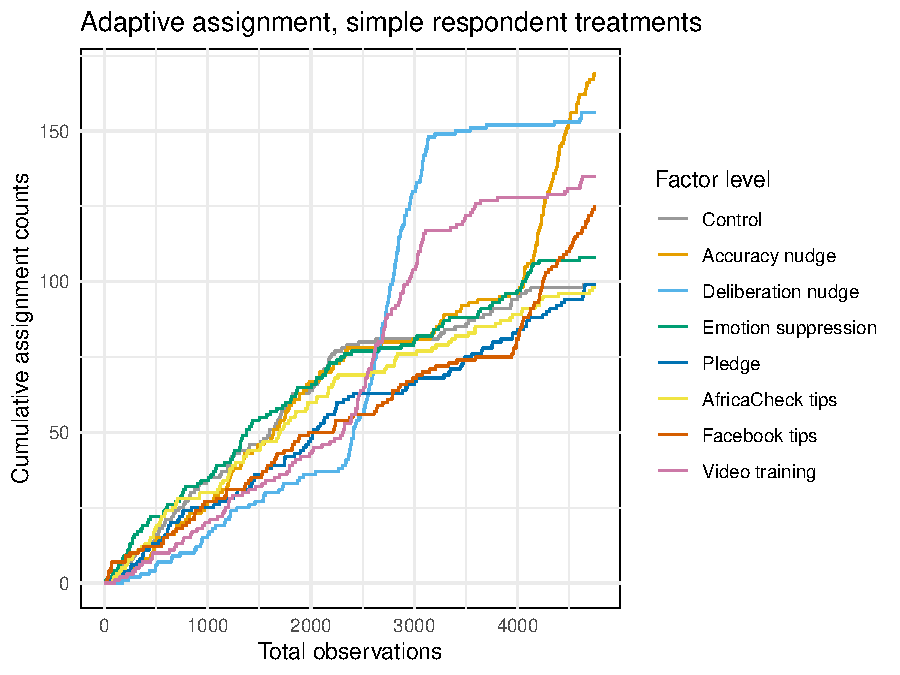
\includegraphics[width = 0.95\textwidth]{../analysis/figures/respondent_base_assignment_on_time.pdf}
    \end{subfigure}%
    \begin{subfigure}[b]{0.5\textwidth}
        \centering
        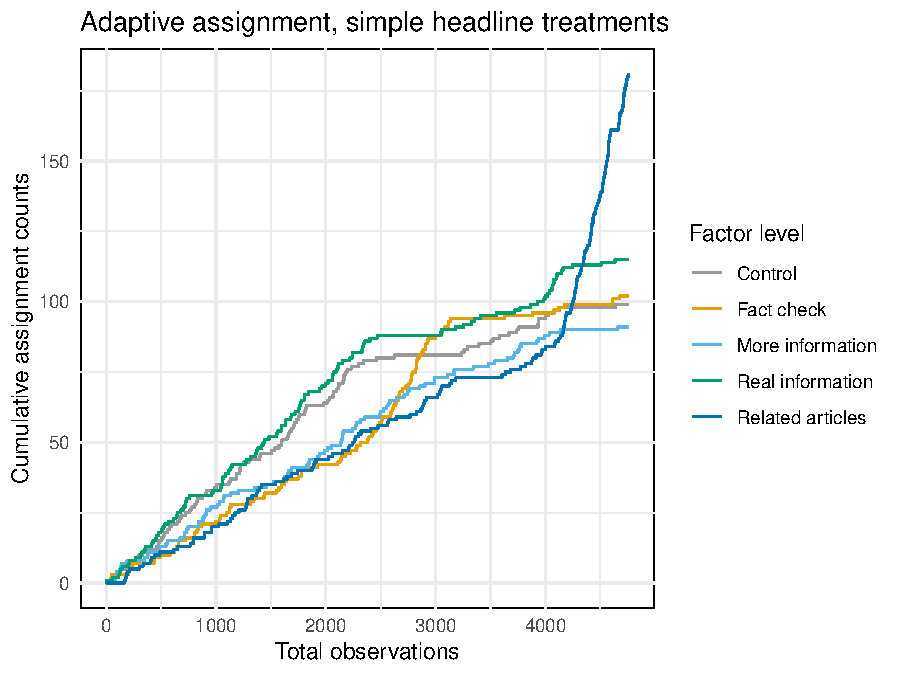
\includegraphics[width = 0.95\textwidth]{../analysis/figures/headline_base_assignment_on_time.pdf}
    \end{subfigure}
   \caption{\textbf{Cumulative treatment assignment during the learning phase for headline (left panel) and respondent (right panel) interventions.} While the full design allows for all factor combinations, these plots illustrate assignment using the ``pure'' version of each factor, i.e., when the other factor is at the baseline control condition.}
   \label{fig:learning_cumulative}
\end{figure}\todo{show something about the bayesian posteriors too?}


The adaptive assignment privileges assignment to those interventions that are predicted to be most effective, down-weighting assignment to interventions that are predicted to perform poorly. This means that we collect more data about the interventions that are the most likely to succeed. It is important to note that adaptively collected data introduces additional challenges for policy learning \citep{zhan2021policy}; the exploitation of the bandit can eventually result in extreme probabilities of treatment assignment. However, this exploitation is an important ethical consideration in a setting where we are concerned about avoiding ``backfire'' from counter-productive interventions. The adaptive algorithm allows us to minimize these potentially harmful effects. %(Figure S4 shows that our adaptive design achieves lower regret compared to a standard static experimental design.)

\todo{TK: additional results. @Molly suggests we pin down results in main text first, then add additional material here. }
\end{document}